\documentclass{llncs}

\usepackage{amsmath,amssymb,amsfonts}
\usepackage{graphicx}
\usepackage{xcolor}
\usepackage{stmaryrd}
\usepackage{subcaption}
\usepackage{hyperref,cleveref}
\usepackage{tikz}

\usetikzlibrary{automata,positioning,shapes.multipart}

\title{Flexible Runtime Security Enforcement with Tagged C}
\author{Sean Anderson \and Allison Naaktgeboren \and Andrew Tolmach}
\institute{Portland State University}

\begin{document}

\newcommand{\tagcolor}{C}

\newcommand{\vt}{\mathit{vt}}
\newcommand{\pt}{\mathit{pt}}
\newcommand{\lt}{\mathit{lt}}
\newcommand{\lts}{\overline{\lt}}
\newcommand{\nt}{\mathit{nt}}
\newcommand{\PCT}{\mathcal{P}}

\newcommand{\trule}[2]{#1 \leftarrow #2}

\newcommand{\truledef}[1]{
  & \multispan{3} \(#1\) \\}

\newcommand{\assert}[1]{& & & \multispan{2} \(\mathbf{assert} ~ #1\) \hfill \\}
\newcommand{\letin}[1]{& & & \multispan{2} \(\mathit{let} ~ #1 ~ \mathit{in}\) \\}

\newcommand{\caseof}[1]{\textnormal{case } #1 \textnormal{ of}}
\newcommand{\caseentry}[2]{& & & #1 \Rightarrow #2}

\newcommand{\optional}[1]{\fcolorbox{black}{gray!20}{#1}}
\newcommand{\settag}[2]{\boldsymbol{#1} & \longleftarrow & & \mathit{#2}\\}
\newcommand{\settagopt}[2]{\optional{\(\boldsymbol{#1}\)} & \longleftarrow & & \mathit{#2}\\}

%%% Tag Rules %%%
\newcommand{\loadtname}{\mathbf{LoadT}}
\newcommand{\loadtargs}{\PCT, \pt, \vt, \overline{\lt}}
\newcommand{\loadtres}{\vt'}
\newcommand{\loadt}{\loadtname(\loadtargs)}

\newcommand{\storetname}{\mathbf{StoreT}}
\newcommand{\storetargs}{\PCT, \pt, \vt_1, \vt_2, \overline{\lt}}
\newcommand{\storetres}{\PCT',\vt',\overline{\lt}'}
\newcommand{\storet}{\storetname(\storetargs)}

\newcommand{\consttname}{\mathbf{ConstT}}
\newcommand{\consttres}{\vt}
\newcommand{\constt}{\consttname}

\newcommand{\unoptname}{\mathbf{UnopT}}
\newcommand{\unoptargs}{\PCT, \vt}
\newcommand{\unoptres}{\vt}
\newcommand{\unopt}{\unoptname(\unoptargs)}

\newcommand{\binoptname}{\mathbf{BinopT}}
\newcommand{\binoptargs}{\PCT, \vt_1, \vt_2}
\newcommand{\binoptres}{\vt'}
\newcommand{\binopt}{\binoptname(\binoptargs)}

\newcommand{\globaltname}{\mathbf{GlobalT}}
\newcommand{\globaltargs}{id, s}
\newcommand{\globaltargstyped}{id \in ident, s \in \mathbb{N}}
\newcommand{\globaltres}{\pt,\vt,\overline{\lt}}
\newcommand{\globalt}{\globaltname(\globaltargs)}

\newcommand{\localtname}{\mathbf{LocalT}}
\newcommand{\localtargs}{\PCT, id, s}
\newcommand{\localtargstyped}{\PCT, id \in ident, s \in \mathbb{N}}
\newcommand{\localtres}{\pt,\vt,\overline{\lt}}
\newcommand{\localt}{\localtname(\localtargs)}

\newcommand{\vartname}{\mathbf{VarT}}
\newcommand{\vartargs}{\PCT, \vt}
\newcommand{\vartres}{\pt}
\newcommand{\vart}{\vartname(\vartargs)}

\newcommand{\malloctname}{\mathbf{MallocT}}
\newcommand{\malloctargs}{\PCT, \vt}
\newcommand{\malloctres}{\PCT',\pt,\optional{\(\vt,\overline{\lt}\)}}
\newcommand{\malloct}{\malloctname(\malloctargs)}

\newcommand{\freetname}{\mathbf{FreeT}}
\newcommand{\freetargs}{\PCT, \vt}
\newcommand{\freetres}{\PCT',\pt,\optional{\(\vt,\overline{\lt}\)}}
\newcommand{\freet}{\freetname(\freetargs)}

\newcommand{\picasttname}{\mathbf{PICastT}}
\newcommand{\picasttargs}{\PCT, \pt, \optional{\(\vt, \overline{\lt}\)}}
\newcommand{\picasttres}{\PCT',\vt}
\newcommand{\picastt}{\picasttname(\picasttargs)}

\newcommand{\ipcasttname}{\mathbf{IPCastT}}
\newcommand{\ipcasttargs}{\PCT, \vt_1, \optional{\(\vt_2, \overline{\lt}\)}}
\newcommand{\ipcasttres}{\PCT',\pt}
\newcommand{\ipcastt}{\ipcasttname(\ipcasttargs)}

\newcommand{\ppcasttname}{\mathbf{PPCastT}}
\newcommand{\ppcasttargs}{\PCT, \pt, \optional{\(\vt, \overline{\lt}\)}}
\newcommand{\ppcasttres}{\PCT',\pt'}
\newcommand{\ppcastt}{\picasttname(\picasttargs)}

\newcommand{\iicasttname}{\mathbf{IICastT}}
\newcommand{\iicasttargs}{\PCT, \vt_1}
\newcommand{\iicasttres}{\PCT',\pt}
\newcommand{\iicastt}{\ipcasttname(\ipcasttargs)}

\newcommand{\splittname}{\mathbf{SplitT}}
\newcommand{\splittargs}{\PCT, \vt, \optional{\(L\)}}
\newcommand{\splittres}{\PCT'}
\newcommand{\splitt}{\splittname(\splittargs)}
           
\newcommand{\jointname}{\mathbf{JointT}}
\newcommand{\jointargs}{\PCT, \optional{\(L\)}}
\newcommand{\jointres}{\PCT'}
\newcommand{\joint}{\jointname(\jointargs)}

\newcommand{\argtname}{\mathbf{ArgT}}
\newcommand{\argtargs}{\PCT, \vt, f, x}
\newcommand{\argtargstyped}{\PCT, \vt, f, x \in ident}
\newcommand{\argtres}{\vt'}
\newcommand{\argt}{\argtname(\argtargs)}

\newcommand{\callerrettname}{\mathbf{CallerRetT}}
\newcommand{\callerrettargs}{\PCT, \PCT', \vt}
\newcommand{\callerrettres}{\vt'}
\newcommand{\callerrett}{\callerrettname(\callerrettargs)}

\newcommand{\calleerettname}{\mathbf{CalleeRetT}}
\newcommand{\calleerettargs}{\PCT, \PCT', \vt}
\newcommand{\calleerettres}{\vt'}
\newcommand{\calleerett}{\calleerettname(\calleerettargs)}

%%%%%%%%%%%%%%%%%

%%% Continuations, States, Values %%%

\newcommand{\kemp}{\mathit{Kemp}}
\newcommand{\kdo}[1]{\mathit{Kdo};~ #1}
\newcommand{\kseq}[2]{\mathit{Kseq} ~ #1; ~ #2}
\newcommand{\kif}[4]{\mathit{Kif}[#1 \mid #2] ~ \mathit{join} ~ #3; ~ #4}
\newcommand{\kwhiletest}[4]{\mathit{KwhileTest}(#1) ~ \{ ~ #2 ~ \} ~ \mathit{join} ~ #3; ~ #4}
\newcommand{\kwhileloop}[4]{\mathit{KwhileLoop}(#1) ~ \{ ~ #2 ~ \} ~ \mathit{join} ~ #3; ~ #4}
\newcommand{\kdowhiletest}[4]{\mathit{KdoWhileTest}(#1) ~ \{ ~ #2 ~ \} ~ \mathit{join} ~ #3; ~ #4}
\newcommand{\kdowhileloop}[4]{\mathit{KdoWhileLoop}(#1) ~ \{ ~ #2 ~ \} ~ \mathit{join} ~ #3; ~ #4}
\newcommand{\kfor}[2]{\mathit{Kfor} ~ #1; ~ #2}
\newcommand{\kforpost}[2]{\mathit{KforPost} ~ #1; ~ #2}
\newcommand{\kcall}[3]{\mathit{Kcall} ~ #1 ~ #2 ~ #3}

\newcommand{\ctx}[1]{ctx \left[#1\right]}

\newcommand{\sstate}[6]{\mathcal{S}\left(f,#2,#3,#4 \mid #5 \gg #6 @ #1\right)}
\newcommand{\estate}[6]{\mathcal{E}\left(f,#2,#3,#4 \mid #5; \gg #6 @ #1\right)}
\newcommand{\cstate}[7]{\mathcal{C}\left(#1,#3,#4 \mid #5(#6) \gg #7 @ #2\right)}
\newcommand{\rstate}[6]{\mathcal{R}\left(#1,#3,#4 \mid #5 \gg #6 @ #2\right)}
\newcommand{\fstate}[1]{\mathcal{F}\left(#1\right)}

\newcommand{\mem}{m}
\newcommand{\genv}{\mathit{ge}}
\newcommand{\lenv}{\mathit{le}}
\newcommand{\cont}{k}
\newcommand{\stmt}{s}
\newcommand{\expr}{e}
\newcommand{\type}{ty}
\newcommand{\defestate}[1]
           {\estate{\PCT}{\mem}{\genv}{\lenv}{#1}{\cont}}
\newcommand{\defsstate}[1]
           {\sstate{\PCT}{\mem}{\genv}{\lenv}{#1}{\cont}}

\newcommand{\valof}[1]{|#1|}
\newcommand{\deref}[1]{* #1}
\newcommand{\addrof}[1]{\& #1}
\newcommand{\assignop}[3]{#2 ~~ [#1]\!\!= #3}
\newcommand{\postinc}[2]{#2 #1\!\!#1}
\newcommand{\assign}[2]{#1 := #2}
\newcommand{\loc}[2]{\underline{#1}@#2}
\newcommand{\val}[2]{\mathit{#1} @ #2}
\newcommand{\binop}[3]{#2 #1 #3}
\newcommand{\unop}[2]{#1 #2}
\newcommand{\comma}[2]{#1, #2}
\newcommand{\paren}[2]{(#2) (#1)}
\newcommand{\builtin}[2]{\mathit{builtin} ~ #1(#2)}
\newcommand{\var}[1]{#1}
\newcommand{\cast}[2]{(#2) #1}
\newcommand{\call}[2]{#1(#2)}
\newcommand{\condition}[3]{#1 ~ ? ~ #2 ~ : ~ #3}
\newcommand{\sizeof}[1]{\mathtt{size}(#1)}
\newcommand{\alignof}[1]{\mathtt{align}(#1)}

\newcommand{\sskip}{\mathtt{skip}}
\newcommand{\sdo}[1]{#1;}
\newcommand{\sseq}[2]{#1 ~ #2}
\newcommand{\scontinue}{\mathtt{continue}}
\newcommand{\sbreak}{\mathtt{break}}
\newcommand{\sreturn}{\mathtt{return}}
\newcommand{\sifthenelse}[4]{\mathtt{if}(#1) ~ \mathtt{then} ~ #2 ~ \mathtt{else} ~ #3 ~ \mathtt{join} ~ #4}
\newcommand{\swhile}[3]{\mathtt{while}(#1) ~ \mathtt{do} ~ #2 ~ \mathtt{join} ~ #3}
\newcommand{\sdowhile}[3]{\mathtt{do} ~ #2 ~ \mathtt{while} ~ (#1) ~ \mathtt{join} ~ #3}
\newcommand{\sfor}[5]{\mathtt{for}(#1; #2; #3) ~ \mathtt{do} ~ #4 ~ \mathtt{join} ~ #5}
\newcommand{\sswitch}[2]{\mathtt{switch} ~ #1 ~ \{ ~ #2 ~ \}}
\newcommand{\slabel}[2]{#1: ~ #2}
\newcommand{\sgoto}[1]{\mathtt{goto} ~ #1}

\newcommand{\vundef}{\mathbf{undef}}

\newcommand{\tptr}[1]{\mathit{ptr(#1)}}

\newcommand{\judgment}[3][]{
  {\centering
  \smallskip
  \begin{tabular}{c}
    #2 \\
    \hline
    #3
  \end{tabular}{\sc #1}
  \smallskip\par}}

\newcommand{\judgmentbr}[4][]{
  {\centering
  \smallskip
  \begin{tabular}{c}
    #2 \\
    #3 \\
    \hline
    #4
  \end{tabular}{\sc #1}
   \smallskip\par}}

\newcommand{\judgmentbrbr}[5][]{
  {\centering
  \smallskip
  \begin{tabular}{c}
    #2 \\
    #3 \\
    #4 \\
    \hline
    #5
  \end{tabular}{\sc #1}
   \smallskip\par}}

\newcommand{\judgmentbrbrbr}[6][]{
  {\centering
  \smallskip
  \begin{tabular}{c}
    #2 \\
    #3 \\
    #4 \\
    #5 \\
    \hline
    #6
  \end{tabular}{\sc #1}
   \smallskip\par}}

\newcommand{\judgmenttwobr}[6][]{
  {
    \centering
    \smallskip
    \begin{tabular}{c c}
       #2 & #3 \\
       #4 & #5 \\
       \hline
       \multicolumn{2}{c}{#6}
    \end{tabular}{\sc #1}
    \vspace{\belowdisplayskip}\par
  }}

\newcommand{\judgmenttwobrlong}[5][]{
  {
    \centering
    \smallskip
    \begin{tabular}{c c}
       #2 & #3 \\
       \multicolumn{2}{c}{#4} \\
       \hline
       \multicolumn{2}{c}{#5}
    \end{tabular}{\sc #1}
    \vspace{\belowdisplayskip}\par
  }}

\newcommand{\judgmentthreebrlong}[6][]{
  {
    \centering
    \smallskip
    \begin{tabular}{c c c}
       #2 & #3 & #4 \\
       \multicolumn{3}{c}{#5} \\
       \hline
       \multicolumn{3}{c}{#6}
    \end{tabular}{\sc #1}
    \vspace{\belowdisplayskip}\par
  }}

\newcommand{\judgmentthreebrtwo}[7][]{
  {
    \centering
    \smallskip
    \begin{tabular}{c c c}
       #2 & #3 & #4 \\
       \multicolumn{3}{c}{#5 \hfill #6} \\
       \hline
       \multicolumn{3}{c}{#7}
    \end{tabular}{\sc #1}
    \vspace{\belowdisplayskip}\par
  }}

\newcommand{\judgmenttwobrlongbrlong}[6][]{
  {
    \centering
    \smallskip
    \begin{tabular}{c c}
       #2 & #3 \\
       \multicolumn{2}{c}{#4} \\
       \multicolumn{2}{c}{#5} \\
       \hline
       \multicolumn{2}{c}{#6} \\
    \end{tabular}{\sc #1}
    \vspace{\belowdisplayskip}\par
  }}


\newcommand{\judgmentthreebr}[8][]{
  {
    \centering
    \smallskip
    \begin{tabular}{c c c}
       #2 & #3 & #4 \\
       #5 & #6 & #7 \\
       \hline
       \multicolumn{3}{c}{#8}
    \end{tabular}{\sc #1}
    \vspace{\belowdisplayskip}\par
  }}


\newcommand{\judgmenttwo}[4][]{
  {\centering
  \smallskip
  \begin{tabular}{c c}
    #2 & #3 \\
    \hline
    \multicolumn{2}{c}{#4}
  \end{tabular}{\sc #1}
  \smallskip\par}}

\newcommand{\judgmentthree}[5][]{
  {\centering
  \smallskip
  \begin{tabular}{c c c}
    #2 & #3 & #4 \\
    \hline
    \multicolumn{3}{c}{#5}
  \end{tabular}{\sc #1}
  \smallskip\par}}

\newcommand{\judgmentfour}[6][]{
  {\centering
  \smallskip
  \begin{tabular}{c c c c}
    #2 & #3 & #4 & #5 \\
    \hline
    \multicolumn{4}{c}{#6}
  \end{tabular}{\sc #1}
  \smallskip\par}}

\newcommand{\mallocstep}
{\judgmenttwobrlong
    {\(\trule{\malloctres}{\malloct}\)}
    {\(\mem',p \leftarrow \mathit{heap\_alloc} ~ \mathit{size} ~ \mem\)}
    {\(\mem'' = \mem'\left[p + i \mapsto (\vundef,\vt,\lt) \mid 0 \leq i < s\right]\)}
    {\(\defestate{\ctx{\mathit{malloc(\mathit{size}@t)}}}
      \longrightarrow
      \estate{\PCT'}{\mem''}
             {\ctx{\val{p}{\pt}}}{\cont}\)}}

\newcommand{\valofstep}
{\judgmenttwo{\(\mem[l]_{|ty|} = v@\vt@\overline{\lt}\)}
            {\(\trule{\loadtres}{\loadt}\)}
            {\(\estate{\PCT}{\mem}
              {\ctx{\valof{\loc{l}{\pt}}}}{\cont}
              \longrightarrow
              \estate{\PCT}{\mem}
                     {\ctx{\val{v}{\vt'}}}{\cont}\)}}

\newcommand{\assignopstep}
{\judgmenttwobr{\(\mem[l]_{|ty|} = v_1@\vt @\overline{\lt}\)}
  {\(\oplus \in \{+,-,*,/,\%,<<,>>,\&,^\wedge,|\}\)}
  {\(\trule{\loadtres}{\loadt}\)}
  {\(\expr = \assign{\loc{l}{\pt}}
    {\binop{\oplus}
      {\val{v_1}{\vt'}}
      {\val{v_2}{\vt_2}}}\)}
  {\(\defestate
    {\ctx{\assignop{\oplus}{\loc{l}{\pt}}
        {\val{v_2}{\vt_2}}}}
    \longrightarrow
    \defestate
        {\ctx{\expr}}\)}}

\newcommand{\postincstep}
{\judgmentthreebrtwo{\(\mem[l] = v@\vt @\overline{\lt}\)}
               {\(\oplus \in \{+,-\}\)}
               {\(\trule{\loadtres}{\loadt}\)}
               {\(\trule{\consttres}{\constt}\)}
               {\(\expr = \comma{\assign{\loc{l}{\pt}}{\binop{\oplus}{\val{v}{\vt'}}{1@\constt}}}
                 {\val{v}{\vt'}} \)}
               {\(\defestate
                 {\ctx{\postinc{\oplus}
                     {\loc{l}{\pt}}}}
                 \longrightarrow
                 \defestate
                     {\ctx{\expr}}\)}}

\newcommand{\assignstep}
{\judgmenttwobrlong{\(\mem[l]_{|ty|} = v_1@\vt_1@\overline{\lt}\)}
                  {\(\mem' = \mem[l \mapsto v_2@\vt' @\overline{\lt}']\)}
                  {\(\trule{\storetres}{\storet}\)}
                  {\(\defestate
                    {\ctx{\assign{\loc{l}{\pt}}{\val{v_2}{\vt_2}}}}
                    \longrightarrow
                    \estate{\PCT'}{\mem'}
                           {\ctx{\val{v_2}{\vt_2}}}{\cont}\)}}

\newcommand{\varstep}
{\judgmenttwo{\(\lenv[id] = (l,\_,\pt,ty)\)}
  {\(\trule{\vartres}{\vart}\)}
  {\(\defestate{\ctx{\var{id}}}
    \longrightarrow
    \defestate{\ctx{\loc{l}{\pt}}}\)}}

\newcommand{\unopstep}
{\judgmenttwo{\(\left\langle \odot \right\rangle v = v'\)}
            {\(\vt' = \unopt{\PCT}{\vt}\)}
            {\(\defestate{\ctx{\unop{\odot}{\val{v}{\vt}}}}
              \longrightarrow
              \defestate{\ctx{\val{v'}{\vt'}}}\)}}

\newcommand{\binopstep}
{\judgmenttwo{\(v_1 \left\langle \oplus \right\rangle v_2 = v'\)}
            {\(\vt' = \binopt{\PCT}{\vt_1}{\vt_2}\)}
            {\(\defestate{\ctx{\binop{\oplus}{\val{v_1}{\vt_1}}{\val{v_2}{\vt_2}}}}
              \longrightarrow
              \defestate{\ctx{\val{v'}{\vt'}}}\)}}

\newcommand{\dostepa}
{\judgment{}
  {\(\defsstate{\expr;} \longrightarrow
    \estate{\PCT}{\mem}{\expr}{\kdo{\cont}}\)}
}

\newcommand{\dostepb}
{\judgment{}
  {\(\estate{\PCT}{\mem}{\val{v}{\vt}}{\kdo{\cont}} \longrightarrow
    \defsstate{\sskip}\)}
}

\newcommand{\seqstep}
{\judgment{}
  {\(\defsstate{\stmt_1;\stmt_2} \longrightarrow
    \sstate{\PCT}{\mem}{\stmt_1;}{\kseq{\stmt_2}{\cont}}\)}
}

\newcommand{\seqskipstep}
{\judgment{}
  {\(\sstate{\PCT}{\mem}{\sskip}{\kseq{\stmt}{\cont}} \longrightarrow
    \defsstate{\stmt}\)}
}

\newcommand{\seqcontinuestep}
{\judgment{}
  {\(\sstate{\PCT}{\mem}{\scontinue}{\kseq{\stmt}{\cont}} \longrightarrow
    \sstate{\PCT}{\mem}{\scontinue}{\cont}\)}}

\newcommand{\seqbreakstep}
{\judgment{}
  {\(\sstate{\PCT}{\mem}{\sbreak}{\kseq{\stmt}{\cont}} \longrightarrow
    \sstate{\PCT}{\mem}{\sbreak}{\cont}\)}}

\newcommand{\ifstepa}
{\judgment{\(\stmt=\sifthenelse{\expr}{\stmt_1}{\stmt_2}{L}\)}
  {\(\defsstate{\stmt} \longrightarrow
    \estate{\PCT}{\mem}{\expr}{\kif{\stmt_1}{\stmt_2}{L}{\cont}}\)}
}

\newcommand{\ifstepb}
{\judgmenttwo
  {\(\stmt' =
    \begin{cases}
      \stmt_1 & \textnormal{if } \mathit{boolof}(v) = \mathbf{t} \\
      \stmt_2 & \textnormal{if } \mathit{boolof}(v) = \mathbf{f} \\
    \end{cases}\)}
  {\(\trule{\splittres}{\splitt}\)}
  {\(\estate{\PCT}{\mem}{\val{v}{\vt}}{\kif{\stmt_1}{\stmt_2}{L}{\cont}}
    \longrightarrow
    \sstate{\PCT'}{\mem}{\stmt'}{\cont}\)}
}

\newcommand{\whilestep}
{\judgment{\(\stmt=\swhile{\expr}{\stmt'}{L}\)}
  {\(\defsstate{\stmt} \longrightarrow
    \estate{\PCT}{\mem}{\expr}{\kwhiletest{\expr}{\stmt'}{L}{\cont}}\)}
}

\newcommand{\whiletruestep}
{\judgmentthree
  {\(\mathit{boolof}(v) = \mathbf{t}\)}
  {\(\cont_1 = \kwhiletest{\expr}{\stmt}{L}{\cont}\)}
  {\(\cont_2 = \kwhileloop{\expr}{\stmt}{L}{\cont}\)}
  {\(\estate{\PCT}{\mem}{\val{v}{\vt}}{\cont_1}
    \longrightarrow
    \sstate{\PCT'}{\mem}{\stmt}{\cont_2}\)}
}

\newcommand{\whilefalsestep}
{\judgmenttwo
  {\(\mathit{boolof}(v) = \mathbf{f}\)}
  {\(\cont = \kwhiletest{\expr}{\stmt}{L}{\cont'}\)}
  {\(\estate{\PCT}{\mem}{\val{v}{\vt}}{\cont}
    \longrightarrow
    \sstate{\PCT'}{\mem}{\sskip}{\cont'}\)}
}

\newcommand{\whileskipcontinuestep}
{\judgmenttwo{\(\stmt = \sskip \lor \stmt = \scontinue\)}
  {\(\cont = \kwhileloop{\expr}{\stmt}{L}{\cont'}\)}
  {\(\defsstate{\stmt} \longrightarrow
    \sstate{\PCT}{\mem}{\swhile{\expr}{\stmt}{L}}{\cont'}\)}}

\newcommand{\whilebreakstep}
{\judgment{\(\cont = \kwhileloop{\expr}{\stmt}{L}{\cont'}\)}
  {\(\sstate{\PCT}{\mem}{\sbreak}{\cont} \longrightarrow
    \sstate{\PCT}{\mem}{\sskip}{\cont'}\)}}

\newcommand{\dowhilestep}
{\judgmenttwo{\(\stmt = \sdowhile{\expr}{\stmt}{L}\)}
  {\(\cont' = \kdowhileloop{\expr}{\stmt}{L}{\cont}\)}
  {\(\defsstate{\stmt} \longrightarrow
    \sstate{\PCT}{\mem}{\stmt}{\cont'}\)}
}

\newcommand{\dowhileskipcontinuestep}
{\judgmenttwo
  {\(\cont_1 = \kdowhileloop{\expr}{\stmt}{L}{\cont'}\)}
  {\(\cont_2 = \kdowhiletest{\expr}{\stmt}{L}{\cont}\)}
  {\(\sstate{\PCT}{\mem}{\stmt' = \sskip \lor \stmt' = \scontinue}{\cont_1} \longrightarrow
    \estate{\PCT}{\mem}{\expr}{\cont_2}\)}}

\newcommand{\dowhiletruestep}
{\judgmenttwo
  {\(\mathit{boolof}(v) = \mathbf{t}\)}
  {\(\cont = \kdowhiletest{\expr}{\stmt}{L}{\cont'}\)}
  {\(\estate{\PCT}{\mem}{\val{v}{\vt}}{\cont}
    \longrightarrow
    \sstate{\PCT'}{\mem}{\sdowhile{\expr}{\stmt}{L}}{\cont'}\)}
}

\newcommand{\dowhilefalsestep}
{\judgmenttwo
  {\(\mathit{boolof}(v) = \mathbf{f}\)}
  {\(\cont = \kdowhiletest{\expr}{\stmt}{L}{\cont'}\)}
  {\(\estate{\PCT}{\mem}{\val{v}{\vt}}{\cont}
    \longrightarrow
    \sstate{\PCT'}{\mem}{\sskip}{\cont'}\)}
}

\newcommand{\dowhilebreakstep}
{\judgment{\(\cont = \kdowhileloop{\expr}{\stmt}{L}{\cont'}\)}
  {\(\sstate{\PCT}{\mem}{\sbreak}{\cont} \longrightarrow
    \sstate{\PCT}{\mem}{\sskip}{\cont'}\)}}

\newcommand{\forinitstep}
{\judgmenttwo
  {\(\stmt = \sfor{\stmt_1}{\expr}{\stmt_2}{\stmt_3}{L}\)}
  {\(\stmt_1 \not = \sskip\)}
  {\(\defsstate{\stmt} \longrightarrow
  \sstate{\PCT}{\mem}{\stmt_1}{\kseq{\sfor{\sskip}{\expr}{\stmt_2}{\stmt_3}{L}}{\cont}}\)}
}

\newcommand{\forstep}
{\judgment{\(\stmt = \sfor{\sskip}{\expr}{\stmt_2}{\stmt_3}{L}\)}
  {\(\defsstate{\stmt} \longrightarrow
  \estate{\PCT}{\mem}{\expr}{\kfor{\stmt}{\cont}}\)}
}

\newcommand{\forfalsestep}
{\judgment{\(\mathit{boolof}(v) = \mathbf{f}\)}
  {\(\estate{\PCT}{\mem}{\val{v}{\vt}}{\kfor{\stmt}{\cont}} \longrightarrow
    \sstate{\PCT}{\mem}{\sskip}{\cont}\)}
}

\newcommand{\fortruestep}
{\judgmenttwo{\(\stmt = \sfor{\sskip}{\expr}{\stmt_2}{\stmt_3}{L}\)}
             {\(\mathit{boolof}(v) = \mathbf{t}\)}
  {\(\estate{\PCT}{\mem}{\val{v}{\vt}}{\kfor{\stmt}{\cont}} \longrightarrow
      \sstate{\PCT}{\mem}{\stmt_3}{\kfor{\stmt}{\cont}}\)}
}

\newcommand{\forskiporcontinuestep}
{\judgmenttwo{\(\stmt = \sfor{\sskip}{\expr}{\stmt_1}{\stmt_2}{L}\)}
  {\(\stmt = \sskip \lor \stmt = \scontinue\)}
  {\(\sstate{\PCT}{\mem}{\stmt}{\kfor{\stmt}{\cont}}
    \longrightarrow
    \sstate{\PCT}{\mem}{\stmt_1}{\kforpost{\sfor{\sskip}{\expr}{\stmt_1}{\stmt_2}{L}}{\cont}}\)}
}

\newcommand{\forbreakstep}
{\judgment{\(\stmt = \sfor{\sskip}{\expr}{\stmt_1}{\stmt_2}{L}\)}
  {\(\sstate{\PCT}{\mem}{\sbreak}{\kfor{\stmt}{\cont}}
    \longrightarrow
    \sstate{\PCT}{\mem}{\sskip}{\cont}\)}
}
  
\newcommand{\forskippoststep}
{\judgment{\(\stmt = \sfor{\sskip}{\expr}{\stmt_1}{\stmt_2}{L}\)}
  {\(\sstate{\PCT}{\mem}{\sskip}{\kforpost{\stmt}{\cont}}
    \longrightarrow
    \defsstate{\stmt}\)}
}

\newcommand{\callexprstep}
{\judgment{}
  {\(\estate{\PCT}{\mem}{\ctx{\call{f'}{\overline{v @ \vt}}}}{ty}{\cont}
    \longrightarrow
    \cstate{f'}{\PCT}{\mem}{\genv}{\lenv}{v @ \vt}{\kcall{f}{\ctx}{\cont}}\)}
}

\newcommand{\retvalstep}
{\judgment{\(\mathit{pop} ~ \cont = \kcall{f'}{\ctx}{\cont'}\)}
  {\(\sstate{\PCT}{\mem}{\sreturn ~ \val{v}{\vt}}{\cont}
    \longrightarrow
    \rstate{f'}{\PCT}{\mem}{\genv}{\val{v}{\vt}}{\ctx}{\cont}\)}
}

\newcommand{\callstep}
{\judgmentbr{\(\mathit{def}(f) = (xs, \stmt)\)}
  {\(\lenv' = \lenv \llbracket x \mapsto v@\vt' \mid
    (x,v@\vt) \leftarrow \mathit{zip}(xs,args), \vt' \leftarrow \argt \rrbracket\)}
  {\(\cstate{f}{\PCT}{\mem}{\genv}{\lenv}{args}{\cont} \longrightarrow
    \sstate{\PCT}{\mem}{\genv}{\lenv'}{\stmt}{\cont}\)}}

\newcommand{\returnstep}
{\judgmenttwo{\(\cont = \mathit{Kcall} ~ \lenv' ~ \mathit{ctx} ~ \cont'\)}
  {\(\PCT'',\vt' \leftarrow \rett\)}
  {\(\rstate{\PCT}{\mem}{\genv}{\lenv}{\val{v}{\vt}}{\cont} \longrightarrow
    \estate{\PCT'}{\mem}{\mathit{ctx}[\val{v}{\vt'}]}{\cont'}\)}}

\newcommand{\labelstep}
{\judgment
  {\(\jointres \leftarrow \joint \)}
  {\(\sstate{\PCT}{\mem}
    {L: \stmt}{\cont} \longrightarrow
    \sstate{\PCT'}{\mem}{\genv}{\lenv'}{\stmt}{\cont}\)}}

\newcommand{\memory}[4]
           {             
             \begin{tabular}{|c|c|c|c|}
               \multicolumn{4}{l}{#1} \\
               \hline
               \multicolumn{4}{|c|}{#2 \(@\) #3} \\
               \hline
               \footnotesize #4 & \footnotesize #4 & \footnotesize #4 & \footnotesize #4 \\
               \hline
             \end{tabular}
           }
           
\newcommand{\memoryA}
           {
             node {\memory{1000}{\(\vundef\)}{\(\N\)}{\(\N\)}}; \&
             node {\memory{1004}{\(\vundef\)}{\(\N\)}{\(\N\)}}; \&
             node {\memory{1008}{\(\vundef\)}{\(\N\)}{\(\N\)}}; \&
             node {\memory{1092}{\(\vundef\)}{\(\N\)}{\(\N\)}}; \&
             node {\memory{1096}{\(\vundef\)}{\(\N\)}{\(\N\)}}; \\
           }

\newcommand{\truleblock}[2]
           {
             \tcbox{
             \begin{tabular}{l}
               #1 \\
               #2 \\
             \end{tabular}}
           }

\newcommand{\malloctname}{\color{blue} \mathbf{MallocT}}
\newcommand{\malloctargs}{\PCT, \pt, \vt}
\newcommand{\malloctres}{\PCT['],\pt['],\vt['],\lt[']}
\newcommand{\malloct}{\malloctname(\malloctargs)}

\newcommand{\malloctruleblock}[1]
           {
             \truleblock{\(\malloct\)}{#1}
           }

\newcommand{\localtname}{\color{blue} \mathbf{LocalT}}
\newcommand{\localtargs}{\PCT, \TN}
\newcommand{\localtres}{\PCT['], \pt['], \lt[']}
\newcommand{\localt}{\localtname(\localtargs)}

\newcommand{\localtruleblock}[1]
           {
             \truleblock{\(\localt\)}{#1}
           }

\newcommand{\accesstname}{\color{blue} \mathbf{AccessT}}
\newcommand{\accesstargs}{\PCT,\vt}
\newcommand{\accesstres}{\vt[']}
\newcommand{\accesst}{\accesstname(\accesstargs)}

\newcommand{\accesstruleblock}[1]
           {
             \truleblock{\(\accesst\)}{#1}
           }

\newcommand{\loadtname}{\color{blue} \mathbf{LoadT}}
\newcommand{\loadtargs}{\PCT, \pt, \vt, \lt}
\newcommand{\loadtres}{\vt[']}
\newcommand{\loadt}{\loadtname(\loadtargs)}

\newcommand{\loadtruleblock}[1]
           {
             \truleblock{\(\loadt\)}{#1}
           }

\newcommand{\assigntname}{\color{blue} \mathbf{AssignT}}
\newcommand{\assigntargs}{\PCT,\vt[_1],\vt[_2]}
\newcommand{\assigntres}{\PCT['],\vt[']}
\newcommand{\assignt}{\assigntname(\assigntargs)}

\newcommand{\assigntruleblock}[1]
           {
             \truleblock{\(\assignt\)}{#1}
           }
           
\newcommand{\storetname}{\color{blue} \mathbf{StoreT}}
\newcommand{\storetargs}{\PCT, \pt, \vt, \lt}
\newcommand{\storetres}{\PCT['],\vt['],\lt[']}
\newcommand{\storet}{\storetname(\storetargs)}

\newcommand{\storetruleblock}[1]
           {
             \truleblock{\(\storet\)}{#1}
           }

\newcommand{\unoptname}{\color{blue} \mathbf{UnopT}}
\newcommand{\unoptargs}{\odot, \PCT, \vt}
\newcommand{\unoptres}{\vt[']}
\newcommand{\unopt}{\unoptname(\unoptargs)}
           
\newcommand{\unoptruleblock}[2]
           {
             \colorbox{blue!10}{
               \begin{tabular}{l}
                 \(\unopt\) \\
                 % body
                 #1 \\
                 % outputs
                 \{ \(\unoptres\) \} \\
               \end{tabular}
             }
           }
           
\newcommand{\binoptname}{\color{blue} \mathbf{BinopT}}
\newcommand{\binoptargs}{\oplus, \PCT, \vt[_1], \vt[_2]}
\newcommand{\binoptexargs}{\oplus,\vt[_1],\vt[_2]}
\newcommand{\binoptres}{\vt[']}
\newcommand{\binopt}{\binoptname(\binoptargs)}
\newcommand{\binoptex}{\binoptname(\binoptexargs)}

\newcommand{\binoptruleblock}[1]
           {
             \truleblock{\(\binopt\)}{#1}
           }

\newcommand{\binoptexruleblock}[1]
           {
             \truleblock{\(\binoptex\)}{#1}
           }

           
\newcommand{\calltname}{\color{blue} \mathbf{CallT}}
\newcommand{\calltargs}{\PCT, \pt}
\newcommand{\calltres}{\PCT[']}
\newcommand{\callt}{\calltname(\calltargs)}
           
\newcommand{\calltruleblock}[1]
           {
             \truleblock{\(\callt\)}{#1}
           }

\newcommand{\argtname}{\color{blue} \mathbf{ArgT}}
\newcommand{\argtargs}{\PCT, \vt, \FN, \AN}
\newcommand{\argtexargs}{\vt,\FN,\AN}
\newcommand{\argtres}{\PCT['], \vt[']}
\newcommand{\argt}{\argtname(\argtargs)}
\newcommand{\argtex}{\argtname(\argtexargs)}

\newcommand{\argtruleblock}[1]
           {
             \truleblock{\(\argt\)}{#1}
           }

\newcommand{\argtexruleblock}[1]
           {
             \truleblock{\(\argtex\)}{#1}
           }
           
\newcommand{\rettname}{\color{blue} \mathbf{RetT}}
\newcommand{\rettargs}{\PCT[_{\color{blue} CLE}], \PCT[_{\color{blue} CLR}], \vt}
\newcommand{\rettres}{\PCT['],\vt[']}
\newcommand{\rett}{\rettname(\rettargs)}

\newcommand{\rettruleblock}[1]
           {
             \truleblock{\(\rett\)}{#1}
           }

\newcommand{\consttname}{\color{blue} \mathbf{ConstT}}
\newcommand{\consttargs}{\PCT}
\newcommand{\consttres}{\vt[']}
\newcommand{\constt}{\consttname(\consttargs)}

\newcommand{\consttruleblock}[1]
           {
             \truleblock{\(\constt\)}{#1}
           }

\newcommand{\inittname}{{\color{blue} \mathbf{InitT}}}
\newcommand{\inittargs}{\PCT}
\newcommand{\inittres}{\vt[']}
\newcommand{\initt}{\inittname(\inittargs)}

\newcommand{\inittruleblock}[1]
           {
             \truleblock{\(\initt\)}{#1}
           }
           
\newcommand{\globaltname}{\color{blue} \mathbf{GlobalT}}
\newcommand{\globaltargs}{\GN, \TN}
\newcommand{\globaltres}{\pt['],\vt['],\lt[']}
\newcommand{\globalt}{\globaltname(\globaltargs)}

\newcommand{\globaltruleblock}[1]
           {
             \truleblock{\(\globalt\)}{#1}
           }

\newcommand{\dealloctname}{\color{blue} \mathbf{DeallocT}}
\newcommand{\dealloctargs}{\PCT, \TN}
\newcommand{\dealloctres}{\PCT['],\vt['],\lt[']}
\newcommand{\dealloct}{\dealloctname(\dealloctargs)}

\newcommand{\freetname}{\color{blue} \mathbf{FreeT}}
\newcommand{\freetargs}{\PCT,\pt,\vt}
\newcommand{\freetres}{\PCT['],\vt['],\lt[']}
\newcommand{\freet}{\freetname(\freetargs)}

\newcommand{\picasttname}{\color{blue} \mathbf{PICastT}}
\newcommand{\picasttargs}{\PCT, \pt, \lt, \TN}
\newcommand{\picasttres}{\vt[']}
\newcommand{\picastt}{\picasttname(\picasttargs)}

\newcommand{\picasttruleblock}[1]
           {
             \truleblock{\(\picastt\)}{#1}
           }

\newcommand{\ipcasttname}{\color{blue} \mathbf{IPCastT}}
\newcommand{\ipcasttargs}{\PCT, \vt, \lt, \TN}
\newcommand{\ipcasttres}{\pt[']}
\newcommand{\ipcastt}{\ipcasttname(\ipcasttargs)}

\newcommand{\ipcasttruleblock}[1]
           {
             \truleblock{\(\ipcastt\)}{#1}
           }

\newcommand{\ppcasttname}{\color{blue} \mathbf{PPCastT}}
\newcommand{\ppcasttargs}{\PCT, \pt[_1], \pt[_2], \lt[_1], \lt[_2], \TN}
\newcommand{\ppcasttres}{\pt[']}
\newcommand{\ppcastt}{\ppcasttname(\ppcasttargs)}

\newcommand{\iicasttname}{\color{blue} \mathbf{IICastT}}
\newcommand{\iicasttargs}{\PCT, \vt[_1], \TN}
\newcommand{\iicasttres}{\pt[']}
\newcommand{\iicastt}{\iicasttname(\iicasttargs)}

\newcommand{\splittname}{\color{blue} \mathbf{SplitT}}
\newcommand{\splittargs}{\PCT, \vt, \LN}
\newcommand{\splittres}{\PCT[']}
\newcommand{\splitt}{\splittname(\splittargs)}

\newcommand{\splittruleblock}[1]
           {
             \truleblock{\(\splitt\)}{#1}
           }

\newcommand{\exprsplittname}{\color{blue} \mathbf{ExprSplitT}}
\newcommand{\exprsplittargs}{\PCT, \vt}
\newcommand{\exprsplittres}{\PCT[']}
\newcommand{\exprsplitt}{\exprsplittname(\exprsplittargs)}

\newcommand{\exprsplittruleblock}[1]
           {
             \colorbox{blue!10}{
               \begin{tabular}{l}
                 \(\exprsplitt\) \\
                 #1 \\
               \end{tabular}
             }
           }


\newcommand{\exprjointname}{\color{blue} \mathbf{ExprJoinT}}
\newcommand{\exprjointargs}{\PCT, \vt}
\newcommand{\exprjointres}{\PCT['], \vt[']}
\newcommand{\exprjoint}{\exprjointname(\exprjointargs)}

\newcommand{\exprjointruleblock}[1]
           {
             \colorbox{blue!10}{
               \begin{tabular}{l}
                 \(\exprjoint\) \\
                 #1 \\
               \end{tabular}
             }
           }

\newcommand{\labeltname}{\color{blue} \mathbf{LabelT}}
\newcommand{\labeltargs}{\PCT, \LN}
\newcommand{\labeltres}{\PCT[']}
\newcommand{\labelt}{\labeltname(\labeltargs)}

\newcommand{\labeltruleblock}[1]
           {
             \truleblock{\(\labelt\)}{#1}
           }

\newcommand{\extcalltname}{\color{blue} \mathbf{ExtCallT}}
\newcommand{\extcalltargs}{\PCT, \pt, \overline{\vt}}
\newcommand{\extcalltres}{\PCT[']}
\newcommand{\extcallt}{\extcalltname(\extcalltargs)}

\newcommand{\fieldtname}{\color{blue} \mathbf{FieldT}}
\newcommand{\fieldtargs}{\PCT, \pt, \TN, \GN}
\newcommand{\fieldtres}{\pt[']}
\newcommand{\fieldt}{\fieldtname(\fieldtargs)}

%%%%%%%%%%%%%%%%%

\newcommand{\caseofthree}[7]
           {
             \begin{tabular}{l c l}
               \multicolumn{3}{l}{\textnormal{case } #1 \textnormal{ of}} \\
               #2 & \(\Rightarrow\) & #3 \\
               #4 & \(\Rightarrow\) & #5 \\
               #6 & \(\Rightarrow\) & #7 \\
             \end{tabular}
           }

\newcommand{\caseoftwo}[5]
           {
             \begin{tabular}{l c l}
               \multicolumn{3}{l}{\textnormal{case } #1 \textnormal{ of}} \\
               #2 & \(\Rightarrow\) & #3 \\
               #4 & \(\Rightarrow\) & #5 \\
             \end{tabular}
           }


\begin{abstract}
Today's computing infrastructure is built atop layers of legacy C code, often
insecure, poorly understood, and/or difficult to maintain.
These foundations may be shored up with dynamic security enforcement,
which spares legacy code owners from having to modify their code.
% and potentially introduce regressions.
Tagged C is a C variant with a built-in {\em tag-based reference monitor} for use in expressing
a variety of dynamic security policies and enforcing them with compiler and hardware support.

Tagged C is comprehensive in the policies that it can support. In this paper we will discuss
{\em memory safety}, {\em compartmentalization}, and {\em secure information flow} (SIF)
policies. It is flexible in covering the tradeoff between conservative policies that may
halt too many programs and more permissive ones. And as a source language, it should be
more accessible to C programmers than existing assembly-level tag-based reference monitors.

\end{abstract}

\maketitle

\section{Introduction}
Many essential technologies rely on new and old C code. 
Operating systems (Linux, Windows, OSX, BSD), databases (Oracle, sqlite3), the internet \&
web (Apache, NGNIX, NetBSD, Cisco IOS), the Internet of Things (IoT), and the 
embedded devices that run our homes and hospitals are built in and on C \cite{Munoz:PoweredbyC}. 
C is not a relic; more than a third of professional programmers report active developing
in C today \cite{stackoverflow22:dev-survey}. The safety of public and private systems we depend on every day
in turn depends on the security of their underlying C codebases. Insecurity might take the form
of undefined behavior such as memory errors, of logic errors such as sql injection or other
input-sanitization flaws, or of larger-scale architectural flaws that over-provision components of the
system with privilege.

%AMN - not everyone will agree on what is secure behavior, 
% esp as we can't even agree on what defined C is, so give poeple the tools to specficy themselves
% and the tools to change it later on.  
The last line of defense against unknown or unfixable vulnerabilities is dynamic enforcement at
runtime. To this end, we introduce Tagged C: a general-purpose dynamic tag-based enforcement language
that allows developers to define flexible security policies on top of their existing C codebases,
from defining memory UB to specifying detailed information flow policies.

\apt{... the para makes it sound like we are only interested in C language errors. 
  But bugs in the programmer's logic are at least as important for the properties we are trying to enforce!}
\amn{I thought the focus was on C UB limiting and thats kinda C specific? Are there logic errors
  in any of our example sections?}
\sna{SQL injection and information leaks are logic errors}

A tag-based reference monitor associates a metadata tag with the data in the underlying system,
and throughout execution it updates these tags according to a set a predefined rules, or halts if
the program would violate a rule, replacing a security violation with failstop behavior. By attaching
such a monitor to the C language, we allow a user to apply whatever security policy meets their needs,
tuned if necessary so that non-standard but benign code can still run, while actually dangerous activity
is halted.

\sna{Explicitly call out that we can change things without recompilation}

Tagged C consists of an underlying semantics that establishes the baseline concrete behavior of programs
with no policies, and a set of {\em control points} at which the semantics consult a user defined set of
{\em tag rules}. Our underlying semantics are built on the CompCert C semantics, the C semantics formalized
along with the CompCert verified compiler \cite{Leroy09:CompCert}. We provide a reference interpreter
also based on that of CompCert.
\sna{I feel some need to justify this, but I'm not sure what justification is appropriate.}
%Our interpeter is likewise built on top of the CompCert C reference interpreter .
%We chose CompCert C as a base because it is a widely used\apt{??} and well-supported\apt{??} C semantics, with a working
%interpreter and a full formalization. Being written in Coq, it is ideal for future proof work.\apt{why is this relevant?}

\sna{I'm organizing our diss tracks into paragraphs that we can cut or move as needed}
\paragraph*{Why Dynamic?}
  
  Unfortunately, it is not always possible to fully secure C code before run-time.
  Ideally, bugs would be quickly identified and then fixed promptly. 
  That is not always possible for a variety of reasons: bugs may escape detection, 
  require significant effort to diagnose, or be impractical to fix. 
  There are many techniques for finding bugs, but there is a shared stumbling block: C is not 
  well defined. We cannot always agree on when something is a bug in C, especially code using
   Undefined Behaviors (UB) \cite{defactoC}. Confusion around expected behavior is no small problem. 
  There are 191 undefined behaviors and 52 unspecified behaviors in the C99 
  specification \cite{Csmith}. Sometimes these behaviors are benign and skillfully 
  used by the developer, other times they are unintended and highly dangerous. 
  Unfortunately the distinction between the two is easily lost. 
  Discerning expert code review is considered best practice, although it is 
  rarely perfectly successful \cite{} % https://dl.acm.org/doi/10.1007/978-3-642-36563-8_14 }
  even if an expert is available at all. Even when there is both consensus 
  and detection of a bug\apt{??} \amn{we can find it at and we can agree its a problem that should be fixed}, 
  changing the code may not be possible because  
  it is in proprietary 3rd party libraries and drivers, or because
  regulations prohibit changes \cite{Bessey10:Coverity}.

  \apt{last clause is mysterious} \amn {
    for example FDA approval used to forbid patching because you'd have to go through recertification. 
    So healthcare wouldn't patch. SNA pointed out the coverity paper comments on this as a reason for 
    bugs not getting fixed}


\paragraph*{Why C-Level?}
Tag-based enforcement in general has a significant body of work at the assembly level, especially
PIPE (Programmable Interlocks for Policy Enforcement) \cite{}. However, even at the assembly-level
these systems need the compiler to be in the trusted computing base (TCB), as many policies require
knowledge of source-level constructs, even ones that do not depend on detailed knowledge of the program's
behavior [cite Nick and Andre; anyone else?]. Moving policy-definition to the source level therefore
does not expand the TCB and allows C developers to reason about policies in terms of the language that
they program in regularly.

%This is the underlying concept of PIPE, an ISA extension that implements a reference monitor in
%hardware, as well as similar systems such as ARM MTE and [that thing from Binghamton]. Being
%implemented at the ISA level, these systems currently require their policies to be defined in terms of
%assembly code, usually with the help of a compiler. Instead, we attach tags to the C language
%itself, and aim to use PIPE as a compilation target, translating the high-level tags into
%PIPE's ISA primitives.

\paragraph{Contributions}

We offer the following contributions:

\begin{itemize}
\item A full formal semantics for Tagged C, formalized in Coq
\item A complete set of {\em control points} at which the language interfaces with the policy
\item A Tagged C interpreter, implemented in Coq and extracted to Ocaml
\item Policies implementing (1) compartmentalization,
  (2) realistic, permissive memory models from the literature (PVI and PNVI),
  and (3) Secure Information Flow (SIF)
\end{itemize}

In the next section, we give a high-level introduction of metadata-tagging: how it works,
and how that can improve security. Then in \cref{sec:semantics}, we briefly discuss the
language as a whole, before moving into policies in \cref{sec:policies}. Finally, in
\cref{sec:evaluations} we discuss the degree to
which the design meets our goals of flexibility and applicability to realistic
security concerns.

\section{What is Metadata Tagging?}

\apt{I think this example works pretty well, but diagrams are not clear yet.}
  
Consider a very simple security requirement: ``do not {\tt printf} the password.''
For simplicity, we will suppose that {\tt pwd} is an integer in this case.

\vspace{\abovedisplayskip}
\begin{minipage}{0.4\textwidth}
\begin{verbatim}
void main(int pwd) {
  int x = pwd;
  printf("%d", x);
}
\end{verbatim}
\end{minipage}
\begin{minipage}{0.6\textwidth}
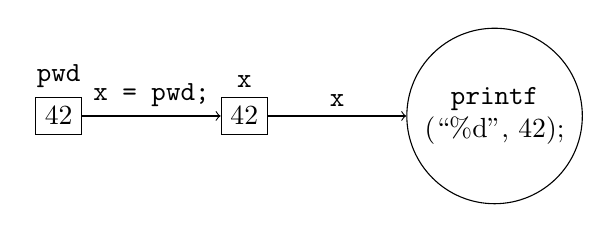
\begin{tikzpicture}[every text node part/.style={align=center}]
  \node[draw=black]                                  (p)      {\(42\)};
  \node[node distance=0em, above=of p]               (pname)  {\tt pwd};
  \node[node distance=5em, right=of p, draw=black]   (x)      {\(42\)};
  \node[node distance=0em, above=of x]               (xname)  {\tt x};
  \node[node distance=5em, right=of x, state]        (printf) {\tt printf \\ (``\%d'', 42);};

  \path[->]
  (p) edge node [pos=0.5,above] {\tt x = pwd;} (x)
  (x) edge node [pos=0.5,above] {\tt x}        (printf);
\end{tikzpicture}
\end{minipage}
\vspace{\belowdisplayskip}

\apt{Not clear what the labels on edges mean.  (And why is there a font change in the figure?)}

We need a way to dynamically track the confidential status of {\tt pwd} as it moves through the variable
{\tt x} and is then passed to {\tt printf}. We can do so by associating metadata with the
value; namely, that it originates in {\tt pwd}. We will write this ``tagged'' value \(42 @ \PT\),
with the \(@\) symbol denoting a value tagged with metadata.
All other values will be tagged \(\N\), for ``not {\tt pwd}.''
Then when we copy {\tt pwd} into {\tt x}, it will bring its tag with it unchanged,
as represented by the pattern \(\gentag \rightarrow \gentag\) under the arrow.
When we call {\tt printf}, we must check that the tag is \(\N\), and if it is
\(\PT\), we would like to failstop rather than permit the call.

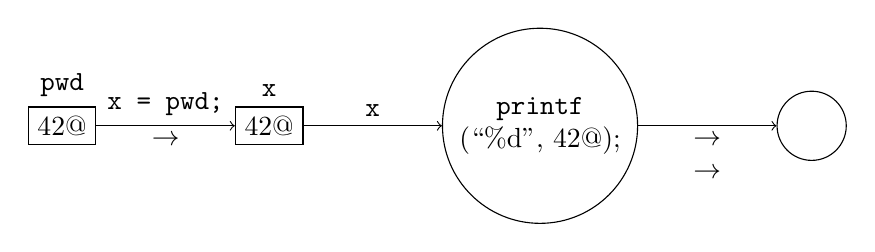
\begin{tikzpicture}[every text node part/.style={align=center}]
  \node[draw=black]                                  (p)      {\(42 @ \PT\)};
  \node[node distance=0em, above=of p]               (pname)  {\tt pwd};
  \node[node distance=5em, right=of p, draw=black]   (x)      {\(42 @ \PT\)};
  \node[node distance=0em, above=of x]               (xname)  {\tt x};
  \node[node distance=5em, right=of x, state]        (printf) {\tt printf \\ (``\%d'', \(42@\PT\));};
  \node[node distance=5em, right=of printf, state]   (fail)   {\(\fail\)};
  
  \path[->]
  (p) edge node [pos=0.5,above] {\tt x = pwd;}
           node [pos=0.5,below] {\(\gentag \rightarrow \gentag\)} (x)
  (x) edge node [pos=0.5,above] {\tt x} (printf)
  (printf) edge node [pos=0.5,above] {}
                node [pos=0.5,below] {\(\N \rightarrow \N\) \\ \(\PT \rightarrow \fail\)} (fail);
\end{tikzpicture}

\apt{Arrow to ``fail'' is confusing. We should only go there is tag on x is P. And it is unclear that the N and P on the
  arrow label are attached to the printed value.}

The points at which the tags are checked and either propagated or updated are termed
{\em control points}, and the particular set of rules that are applied to tags at each
control point is a {\em tag rule}. Collectively, the tag rules form a {\em policy}.

If our goal is to prevent {\tt pwd} from being leaked, our policy should also prevent
values derived from {\tt pwd} from leaking. This means that if we add {\tt pwd} to a
constant, we still keep the result tagged \(\PT\)---otherwise, someone watching our output
could deduce \(\PT\) by subtraction.

\begin{verbatim}
void main(int pwd) {
  printf(pwd+5);
}
\end{verbatim}
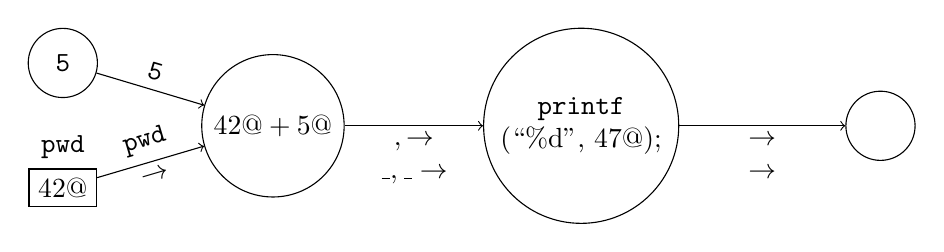
\begin{tikzpicture}[every text node part/.style={align=center}]
  \node[anchor=north]                                     (pname)  {\tt pwd};
  \node[node distance=0em, below=of pname, draw=black]    (p)      {\(42 @ \PT\)};
  \node[node distance=1em, above=of pname, state]         (const)  {\tt 5};
  \node[node distance=5em, right=of pname.north, state]   (sum)    {\(42@\PT + 5@\N\)};
  \node[node distance=5em, right=of sum, state]             (printf) {\tt printf \\ (``\%d'', \(47@\PT\));};
  \node[node distance=6em, right=of printf, state]           (fail)   {\(\fail\)};

  \path[->]
  (p) edge node [pos=0.5,above, sloped] {\tt pwd}
           node [pos=0.5,below, sloped] {\(\gentag \rightarrow \gentag\)} (sum)
  (const) edge node [pos=0.5,above, sloped] {\tt 5}
           node [pos=0.5,below, sloped] {\(\N\)} (sum)
  (sum) edge node [pos=0.5,above] {}
           node [pos=0.5,below] {\(\N,\N \rightarrow \N\) \\ \(\_,\_ \rightarrow \PT\)} (printf)
  (printf) edge node [pos=0.5,above] {}
                node [pos=0.5,below] {\(\N \rightarrow \N\) \\ \(\PT \rightarrow \fail\)} (fail);           
\end{tikzpicture}

Function calls aren't the only means of leaking data, however. We might additionally want
to prevent {\tt pwd} from leaking by being written mmapped memory. Supposing the {\tt mm} is
such a location, we would separately tag the location itself (not just the value in the
location) to designate it as such. We'll call that tag \(\M\). [TODO: the diagrams for this are pretty rough.]

\begin{verbatim}
void main(int pwd) {
  int x = pwd;
  mm = pwd;
}
\end{verbatim}
\begin{tikzpicture}[every text node part/.style={align=center}]
  \node[draw=black]                                  (p)      {\(42 @ \PT\)};
  \node[node distance=0em, above=of p]               (pname)  {\tt pwd};
  \node[node distance=1em, below=of p]   (x0)      {\(\memory{\tt x}{\(\vundef\)}{\(\N\)}{\(\N\)}{}\)};
  \node[node distance=6em, right=of p]   (x)      {\(\memory{\tt x}{42}{\(\PT\)}{\(\N\)}{}\)};
  \node[node distance=2em, right=of x, draw=black]   (p2)      {\(42 @ \PT\)};
  \node[node distance=0em, above=of p2]               (p2name)  {\tt pwd};
  \node[node distance=1em, below=of p2]   (mm0)      {\(\memory{\tt mm}{\(\vundef\)}{\(\N\)}{\(\M\)}{}\)};
  \node[node distance=5em, right=of p2, state]   (fail)   {\(\fail\)};
  
  \path[->]
  (p) edge node [pos=0.5,above] {\tt x = pwd;}
  node [pos=0.5,below] {\(\PT,\M \rightarrow \fail\) \\ \(\gentag_1,\gentag_2 \rightarrow \gentag_1,\gentag_2\)} (x)
  (p2) edge node [pos=0.5,above] {\tt mm = pwd;}
  node [pos=0.5,below] {\(\PT,\M \rightarrow \fail\) \\ \(\gentag_1,\gentag_2 \rightarrow \gentag_1,\gentag_2\)} (fail);
\end{tikzpicture}

Finally, we may be concerned with implicit leaks of {\tt pwd}, such as this one:
\begin{verbatim}
void main(int pwd) {
  for (int i; i<pwd; i++) {
    printf(i);
  }
}
\end{verbatim}

This will give away the exact value of {\tt pwd}! In order to prevent this, we must keep track of
when we are inside of a loop or conditional that depends on {\tt pwd}.
To this end, we carry an additional tag associated with the global state. This is called the PC Tag,
written \(\PCT\). In examples that show states we will note it alongside the statement under focus.

\paragraph{PIPE Backend Implementation}

In \cref{Chhak21:Tagine}, Chhak et al. introduce a verified compiler from a toy
high-level language with tags
to a control-flow-graph-based intermediate representation with a PIPE-based
ISA. \apt{Oops. What's PIPE?} This establishes a proof-of-concept for compiling a source language's tag policy to
realistic hardware. They take advantage of the fact that, like everything else in a PIPE system,
instructions in memory carry tags. Instruction tags are statically determined at compile-time.
They ``piggyback'' information about source-level control points onto the tags of the instructions
that implement those source constructs.

\apt{Not clear this belongs in the intro.}
Tagged C is designed to be implemented in the same way. But, before we can soundly transmit
tag rules from the source language to the assembly level, we also need to protect the basic
control-flow properties of the source language. So, a compiled Tagged C requires a backend that
can at the very least protect its control flow. In the case of a PIPE-based backend, we would
run a basic stack-and-function-pointer-safety policy in parallel with whatever Tagged C policy
the user has provided.

\section{The Language}

Tagged C uses the full syntax of CompCert C \cite{Leroy09:CompCert} with minimal modification (\cref{fig:syntax}).
There are two notable syntactical differences in the language, relative to CompCert C:
conditionals and loops take an optional {\em join point} label, and parenthetical expressions
an optional ``context tag.''

Our semantics are a small-step reduction semantics which differ from CompCert C's in
two key respects. These are given in full in the appendix. First, Tagged C's semantics contain
{\em control points}: hooks within the
operational semantics at which the tag policy is consulted and either tags are updated, or the system
failstops. (Control points resemble ``advice points'' in aspect-oriented programming, but narrowly
focused on the manipulation of tags.) A control point consists of the name of a {\em tag rule}
and the bindings of its inputs and outputs; a tag rule is a partial function. The names and
signatures of the tag rules, and their corresponding control points, are listed in \Cref{fig:controlpoints}.

Second, there is no memory-undefined behavior: the source semantics reflect a
concrete target-level view of memory as a flat address space. Without memory safety, programs
that exhibit memory-undefined behavior will act as their compiled equivalents would, potentially
corrupting memory; we expect that a memory safety policy will be a standard default, but that the
strictness of the policy may need to be tuned for programs that use low-level idioms.

The choice of control points and their associations with tag rules, as well as the tag rules'
signatures, are a crucial design element. Our proposed design is sufficient for the three classes of
policy that we explore in this paper, but it may not be complete.

\paragraph{Notations}
\label{sec:semantics}

Values are ranged over by \(v\), variable identifiers by \(x\), and function identifiers by \(f\).
Tags use a number of metavariables: \(t\) ranges over all tags, while we will use
\(\vt\) to refer to the tags associated with values, \(\pt\) for tags on pointer values
and memory-location expressions, \(\lt\) for tags associated with memory locations themselves,
\(\nt\) for ``name tags'' automatically derived from identifiers, \(\PCT\) for the
global ``program counter tag'' or PC Tag.
An {\it atom} is a pair of a value and a tag, \(\val{v}{\vt}\); the @ symbol should be read
as a pair in general, and is used when the second object in the pair is a tag.
Expressions are ranged over by \(\expr\) (Figure \ref{fig:syntax}),
statements by \(\stmt\), and continuations by \(\cont\).
The continuations are defined in \cref{app:continuations}, and step rules in \cref{app:rules}.

Global environments, ranged over by \(\genv\), map identifiers to either function
or global variable definitions, including the variable's location in memory. Local environments,
ranged over by \(\lenv\), map identifiers to atoms.
Memories \(\mem\) map integers to
triples: a value, a ``value tag'' \(\vt\), and a list of ``location tags'' \(\lts\).

A memory is an array of bytes, where each byte is part of an atom.
Each byte is also associated with a ``location tag'' \(\lt\). When a contiguous region of \(s\) bytes
starting at location \(l\) comprise an atom \(v@\vt\), and their locations tags comprise the list \(\lts\),
we write \(\mem[l]_s = v@\vt @\lts\). Likewise, \(\mem[l \dots l + s \mapsto v@\vt @ \lts]_s\)
denotes storing that many bytes. Visually, we will represent whole atoms in memory as condensed boxes,
with their location tags separate. For example, a four-byte aligned address:

\begin{tabular}{|c|c|c|c|}
  \multicolumn{4}{l}{\(l\)} \\
  \hline
  \multicolumn{4}{|c|}{\(v @ \vt\)} \\
  \hline
  \(\lt_1\) & \(\lt_2\) & \(\lt_3\) & \(\lt_4\) \\
  \hline
\end{tabular}

States can be of several kinds, denoted by their script prefix: a {\em general state} \(\mathcal{S}(\dots)\),
an {\em expression state} \(\mathcal{E}(\dots)\), a {\em call state} \(\mathcal{C}(\dots)\), or a
{\em return state} \(\mathcal{R}(\dots)\). Finally, the special state {\em failstop} (\(\mathcal{F}(\dots)\))
represents a tag failure, and carries the state that produced the failure.
[Allison: to whatever degree you've figured out what is useful here by publication-time, we can
  tune this to be more specific.]

\[\begin{aligned}
S ::= & \sstate{\PCT}{\mem}{\stmt}{\cont} \\
| & \estate{\PCT}{\mem}{\expr}{\cont} \\
| & \cstate{f}{\PCT}{\mem}{\lenv}{f'}{\overline{\val{v}{\vt}}}{\cont} \\
| & \rstate{\PCT}{\mem}{\genv}{\lenv}{\val{v}{\vt}}{\cont} \\
| & \fstate{S} \\
\end{aligned}\]

\section{Tags and Policies}
\label{sec:policies}

\begin{table}
  \begin{tabular}{|l|l|l|l|}
    \hline
    Name & Inputs & Outputs & Control Points \\
    \hline
    \(\globaltname\)    & \(\globaltargstyped\)  & \(\globaltres\)    & Program initialization \\
    \(\fieldtname\)     & \(\fieldtargs\)        & \(\fieldtres\)     & Field Access \\
    \(\loadtname\)      & \(\loadtargs\)         & \(\loadtres\)      & ValOf, AssignOp, PostIncr \\
    \(\storetname\)     & \(\storetargs\)        & \(\storetres\)     & Assign \\
    \(\consttname\)     &                        & \(\consttres\)     & Const, PostIncr \\
    \(\unoptname\)      & \(\unoptargs\)         & \(\unoptres\)      & Unary Operation \\
    \(\binoptname\)     & \(\binoptargs\)        & \(\binoptres\)     & Binary Operation \\
    \(\malloctname\)    & \(\malloctargs\)       & \(\malloctres\)    & Call to {\tt malloc} \\
    \(\freetname\)      & \(\freetargs\)         & \(\freetres\)      & Call to {\tt free} \\
    \(\picasttname\)    & \(\picasttargs\)       & \(\picasttres\)    & Cast from pointer to scalar \\
    \(\ipcasttname\)    & \(\ipcasttargs\)       & \(\ipcasttres\)    & Cast from scalar to pointer \\
    \(\ppcasttname\)    & \(\ppcasttargs\)       & \(\ppcasttres\)    & Cast between pointers \\
    \(\iicasttname\)    & \(\iicasttargs\)       & \(\iicasttres\)    & Cast between scalars \\
    \(\exprsplittname\) & \(\exprsplittargs\)    & \(\exprsplittres\) & Control-flow split points in expressions \\
    \(\exprjointname\)  & \(\exprjointargs\)     & \(\exprjointres\)  & Parenthetical expressions \\
    \(\splittname\)     & \(\splittargs\)        & \(\splittres\)     & Split points (\cref{fig:splits})\\
    \(\labeltname\)     & \(\labeltargs\)        & \(\labeltres\)     & Label \\
    \(\calltname\)      & \(\calltargs\)         & \(\calltres\)      & Call \\
    \(\extcalltname\)   & \(\extcalltargs\)      & \(\extcalltres\)   & External Call \\
    \(\localtname\)     & \(\localtargstyped\)   & \(\localtres\)     & Call \\
    \(\argtname\)       & \(\argtargs\)          & \(\argtres\)       & Call \\
    \(\rettname\)       & \(\rettargs\)          & \(\rettres\)       & Return \\
    \(\dealloctname\)   & \(\dealloctargstyped\) & \(\dealloctres\)   & Return \\
    \hline
  \end{tabular}

  \label{fig:controlpoints}
\end{table}

Tagged C can enforce a wide range of policies, as follows.
A policy consists of a tag type \(\tau\), a default tag inhabiting that type, and an instantiation
of each tag rule identified in \cref{fig:controlpoints}.

For each policy under discussion, we will give a code example of the sort of security
situation in which it might be useful. We will introduce a formal characterization drawn
from the literature of a security property that a correct policy should satisfy.
[TODO: talk about properties somewhere before this?]
Then we will walk through the important tag rules, and the control points that call them,
introducing step rules as needed. Finally, if there are any implementation details that
are necessary to realize a policy, we discuss those.

\paragraph*{Control Points with Side-effects and Optional Arguments}

Chhak et al. \cite{Chhak21:Tagine} give a general strategy for mapping Tagged C's tag rules
onto instructions in a PIPE target. But as they note, translating tag rules in full generality
requires adding extra instructions that may be unnecessary for some policies. The most problematic
situation is when a Tagged-C control point requires a tag from a location that is not read under
a normal compilation scheme or must update tags in locations that would otherwise not be written.

To mitigate this, control points whose compilation would add potentially extraneous instructions
take optional parameters or return optional results. We will explain how the rule should be
implemented in the target if the options are used. If a policy does not make use of the options, it will
be sound to compile without the extra instructions. Optional inputs
and outputs are marked with \(\optional{boxes}\).

\paragraph*{Name Tags}

When we want to define a per-program policy, we need to be able to attach tags to the program's
functions, globals, and so on. We do this by automatically embedding their identifiers in tags,
which are available to all policies. These are called {\em name tags} and are ranged over by
\(\nt\). We give name tags to the following constructions and identify them as follows:
\begin{itemize}
\item Function identifiers, \(FN(f)\)
\item Function arguments, \(AN(f,x)\)
\item Global variables, \(GN(x)\)
\item Labels, \(LN(L)\)
\item Types, \(TN(\type)\)
\end{itemize}

\subsection{Basic Memory Safety}
\label{sec:memsafe}

Let's begin by walking through a common type of policy: memory safety. Variations of memory safety
have been enforced in PIPE at the assembly level already, but what does it look like to enforce it
at the source level? Consider some example code:

\begin{verbatim}
void main() {
  int[1] x;
  int[1] y;
  *x = 0;
  *(x+1) = 0;
}
\end{verbatim}

The above code is undefined behavior in C, because it writes to the address one past the end
of the array pointed to by {\tt x}. Since
{\tt x} and {\tt y} are given adjacent concrete addresses, when the program
writes to the address of {\tt x+1}, it is writing to the address of {\tt y}.
For our example, we'll assume that the stack grows downward from address 100.

We can prevent situations like this using a {\em memory safety} policy, as follows.
We assign to each object in memory a unique ``color'' when it is allocated---in this case,
on entry to the function {\tt main}.

Our set of tags consists of
\(N\), for non-pointers, and pointer ``colors'' \(c \in \mathbb{N}\). The PC Tag
(\(\PCT\)) tracks the next color to allocate, so it's initialized to \(\tagz\), and everything else is \(N\).
\(N\) is the default for constants.

\begin{tikzpicture}[every text node part/.style={align=center}]
  \node[matrix, ampersand replacement=\&, draw=black]  (le)
       {
         \node {\it le}; \\
         \node {\(x \mapsto 92 @ \tagone\)}; \\
         \node {\(y \mapsto 96 @ \tagz\)}; \\
       };

  \node[state, node distance=1em, below=of le]  (stmt)
       {
         \(*x = 0@\N\) \\
         {\color{blue} \(\PCT : \tagtwo\)}
       };
  
  \node[matrix, ampersand replacement=\&, column sep=-1em, node distance=0.5em, below=of stmt]  (mem)
       {
         \node[anchor=north] {\(~ ~\cdots ~ ~\)}; \&
         \node[anchor=center] {\memory{\(92\)}{\(\vundef\)}{\(\N\)}{\(\tagone\)}}; \&
         \node[anchor=center] {\memory{\(96\)}{\(\vundef\)}{\(\N\)}{\(\tagz\)}}; \\
       };

  \node[matrix, ampersand replacement=\&, draw=black, node distance=12em, right=of le]  (le2)
       {
         \node {\it le}; \\
         \node {\(x \mapsto 92 @ \tagone\)}; \\
         \node {\(y \mapsto 96 @ \tagz\)}; \\
       };

  \node[state, node distance=1em, below=of le2]  (stmt2)
       { \\
         \(92 @ \tagone = 0@\N\) \\
         {\color{blue} \(\PCT : \tagtwo\)}
       };
  
  \node[matrix, ampersand replacement=\&, column sep=-1em, node distance=-0.5em, below=of stmt2]  (mem2)
       {
         \node[anchor=north] {\(~ ~\cdots ~ ~\)}; \&
         \node[anchor=center] {\memory{\(92\)}{\(\vundef\)}{\(\N\)}{\(\tagone\)}}; \&
         \node[anchor=center] {\memory{\(96\)}{\(\vundef\)}{\(\N\)}{\(\tagz\)}}; \\
       };

  \draw[->]
  (stmt) -- (stmt2);
  
\end{tikzpicture}


%The call to malloc allocates the region from 1000 to 1039, and returns a pointer to the base
%address, 1000. We consult the policy to determine (1) the tag on the resulting value,
%(2) the updated tags on the allocated memory region, and (3) the updated PC Tag.
%Specifically, we invoke the \(\malloctname\) tag rule, which takes the PC Tag and the tag on
%the size argument and returns these three updated tags.

%\begin{tikzpicture}[]
%  \node[matrix, ampersand replacement=\&, column sep=-0.6em]  (mem)
%       {
%         \node[outer ysep=-5pt] (a) {\(\underbrace{\memory{1000}{\(\vundef\)}{\N}{\tagz}}\)};\\ %\&
%         \node {\memory{\(1004\)}{\(\vundef\)}{\(\N\)}{\(\N\)}}; \&
%         \node {\memory{\(1008\)}{\(\vundef\)}{\(\N\)}{\(\N\)}}; \\
%       };
  
%  \node (state) [node distance=1.2em, above=of a]
%        {\(\sstate{\PCT'=\tagone}{\mem}{\expr=p @ \pt}{}\)};

  
%  \malloctruleblock{}{\(\PCT+1\)}{\(\PCT\)}{\(\N\)}{\(\left[\PCT\right]\)}

%  \draw[->]
%  (pctout.north) |- (state.east);

%  \draw[->]
%  (ptout.west) -- (state.south);

%  \draw[->]
%  (vtout.west) -- (a.east);
  
%  \draw[->]
%  (ltsout) -| (a.south);
%\end{tikzpicture}

%In this case, we tag the pointer and the memory region with the current count, and then
%increment the count. Once the pointer is stored in {\tt x}, our memory is:

%We do the same for allocating {\tt y}, to get the memory:

%\begin{tikzpicture}[]
%  \node[matrix, ampersand replacement=\&, column sep=-0.6em]  (mem)
%       {
%         \node (a) {\memory{\(1000\)}{\(\vundef\)}{\(\N\)}{\(\tagz\)}}; \&
%         \node {\memory{\(1004\)}{\(\vundef\)}{\(\N\)}{\(\tagone\)}}; \&
%         \node {\memory{\(1008\)}{\(\vundef\)}{\(\N\)}{\(\N\)}}; \&
%         \node[anchor=north] {\(~ ~\dots ~ ~\)}; \&
%         \node {\memory{\(1092\)}{\(1004\)}{\(\tagone\)}{\(\N\)}}; \&
%         \node {\memory{\(1096\)}{\(1000\)}{\(\tagz\)}{\(\N\)}}; \\
%       };       
%\end{tikzpicture}

Next, the program stores a 0 to address 1000. The constant 0
takes on the default tag, \(I\). The policy needs to check that
this store is valid, in addition to determining the tags on the value that is stored.
This check is performed by comparing the tag on the pointer to the tags on memory---each
byte being written, in case the pointer is misaligned. Then the tag on the value being stored
is propagated with it into memory, unchanged.
[TODO: arrows aren't pointing to quite the right places right now, but one can imagine.]

\begin{tikzpicture}[every text node part/.style={align=center}]
  \node[matrix, ampersand replacement=\&, draw=black]  (le)
       {
         \node {\(x \mapsto 92 @ \tagone\)}; \\
         \node {\(y \mapsto 96 @ \tagz\)}; \\
       };

  \node[state, node distance=1em, below=of le]  (stmt)
       {
         \(92@\tagone = 0@\N\) \\
         {\color{blue} \(\PCT : \tagtwo\)}
       };
  
  \node[matrix, ampersand replacement=\&, column sep=-1em, node distance=0.5em, below=of stmt]  (mem)
       {
         \node[anchor=north] {\(~ ~\cdots ~ ~\)}; \&
         \node[anchor=center] (x) {\(\underbrace{\memory{\(92\)}{\(0\)}{\(\N\)}{\(\tagone\)}}\)}; \&
         \node[anchor=center] {\(~ ~ \cdots ~ ~\)}; \\
       };

  \storetruleblock{\(\mathbf{assert} ~ \forall \lt \in \lts . \pt = \lt\)}{\(\PCT\)}{\(\vt_2\)}{\(\lts\)}

  \draw[->]
  (pctout) -- (stmt.south);
  \draw[->]
  (vtout) -- (x.east);
  \draw[->]
  (ltsout) |- (x.south);
\end{tikzpicture}
  
\vspace{\abovedisplayskip}

Next, on the last line, we add 1 to {\tt x}, which invokes the \(\binoptname\) tag rule
to combine the tags on the arguments. \(\binoptname\) takes as argument the operation \(\oplus\).
In memory safety terms, we can add a pointer to a non-pointer in either order, and we can subtract
a non-pointer from a pointer (but not the reverse), to yield a pointer to the same object. We can
subtract two pointers to the same object from one another to yield a non-pointer, the offset between them.
All other binary operations are only permitted between non-pointers.

\begin{tikzpicture}[every text node part/.style={align=center}]
  \node[matrix, ampersand replacement=\&, draw=black]  (le)
       {
         \node {\(x \mapsto 92 @ \tagone\)}; \\
         \node {\(y \mapsto 96 @ \tagz\)}; \\
       };

  \node[state, node distance=1em, below=of le]  (stmt)
       {
         \(*(x+1) = 0@\N\) \\
         {\color{blue} \(\PCT : \tagtwo\)}
       };
  
  \node[matrix, ampersand replacement=\&, column sep=-1em, node distance=0.5em, below=of stmt]  (mem)
       {
         \node[anchor=north] {\(~ ~\cdots ~ ~\)}; \&
         \node[anchor=center] {\memory{\(92\)}{\(v\)}{\(\N\)}{\(\tagone\)}}; \&
         \node[anchor=center] {\memory{\(96\)}{\(\vundef\)}{\(\N\)}{\(\tagz\)}}; \\
       };

  \node[matrix, ampersand replacement=\&, draw=black, node distance=12em, right=of le]  (le2)
       {
         \node {\(x \mapsto 92 @ \tagone\)}; \\
         \node {\(y \mapsto 96 @ \tagz\)}; \\
       };

  \node[state, node distance=1em, below=of le2]  (stmt2)
       { \\
         \(96 @ \tagone = 0@\N\) \\
         {\color{blue} \(\PCT : \tagtwo\)}
       };
  
  \node[matrix, ampersand replacement=\&, column sep=-1em, node distance=-0.5em, below=of stmt2]  (mem2)
       {
         \node[anchor=north] {\(~ ~\cdots ~ ~\)}; \&
         \node[anchor=center] {\memory{\(92\)}{\(v\)}{\(\N\)}{\(\tagone\)}}; \&
         \node[anchor=center] {\memory{\(96\)}{\(\vundef\)}{\(\N\)}{\(\tagz\)}}; \\
       };

  \draw[->]
  (stmt) -- (stmt2);
  
\end{tikzpicture}


\begin{tikzpicture}       
  \binoptruleblock{}{\(\PCT\)}
                  {\(\left\lbrace \begin{tabular}{l r l}
                      \(c\) & when \((\oplus,~ \vt_1,~ \vt_2)\) is & \(+, c, \N \mid +, \N, c \mid -, c, \N\) \\
                      \(\N\) & is & \(-, c, c \mid \_,\N,\N\) \\
                      \(\fail\) & is & otherwise \\
                    \end{tabular} \right.\)}
\end{tikzpicture}

So, when we try to write through the address \(96@\tagone\), we compare its tag to that of the memory
locations, which are tagged \(\tagz\). Therefore the policy must failstop on the store.

\subsection{PVI Memory Safety}
\label{sec:PVI}

The simple memory safety policy described above is too restrictive to run many real-world
C programs, because they contain undefined behavior that is nevertheless part of the
``de facto standard'' \cite{???}. These low-level idioms are one reason that we might
settle for isolating risky code in a compartment instead of enforcing full memory safety.

Memarian et al. \cite{???} propose two memory models that aim to capture this
de facto standard, support the common low-level idioms, yet still place sufficient
restrictions on programs that it remains sound to use alias analysis in optimizations.
The first of these is {\it PVI} (provenanace via integer), in which pointers remain valid
when they are cast to integers, subjected to the full range of arithmetic operations, and
cast back. Memarian et al. do not propose to enforce PVI, merely to use it as an alternative to the
C standard. But its relative permissiveness makes it a great target for enforcement in Tagged C!
Their second memory model, {\it PNVI} (provenance not via integer), is even more permissive.
We can also enforce it in Tagged C, though its security value is questionable, and we will
not describe it in this paper.

[TODO: For example, garbage collectors use low order bits to mark pointers as in the Cheney algorithm.]

\paragraph*{PVI Definitions}

Since PVI is a more realistic policy than the basic memory safety described above,
we will go into some details elided there. First of all, the distinction between
heap-allocated memory, stack objects, and global variables. The latter are tagged
based on their identifiers, while heap- and stack-objects are tagged dynamically
using unique colors.
%
\begin{align*}
  \tau ::= & \mathit{glob} ~ id & id \in \mathit{ident} \\
  & \mathit{dyn} ~ \tagcolor & \tagcolor \in \mathbb{N} \\
\end{align*}

When initializing program memory, before any execution, each global \(id\) has its
memory locations and its pointer in the global environment tagged with \(\mathit{glob} ~ id\),
using the \(\globaltname\) tag rule.

\[\begin{aligned}
\truledef{\globalt}
\settag{\pt}{\mathit{glob ~ id}}
\settag{\vt}{N}
\settag{\overline{\lt}}{\left[\mathit{glob} ~ id \mid 0 \leq i < s\right]}
\end{aligned}\]

In our previous memory safety example, we began with the active stack frame already allocated.
When it is allocated at runtime, its tags are initialize by the \(\localtname\) rule.
Stack-allocated locals and heap-allocated objects both

The tag rules for allocating memory in the heap and in the stack should look familiar.

\begin{minipage}{0.49\textwidth}
\[\begin{aligned}
\truledef{\localt}
\settag{\pt}{dyn ~ \PCT}
\settagopt{\vt}{N}
\settagopt{\overline{\lt}}{\left[dyn ~ \PCT\right]}
\settag{\PCT'}{\PCT+1}
\end{aligned}\]
\end{minipage}
\begin{minipage}{0.49\textwidth}
\[\begin{aligned}
\truledef{\malloct}
\settag{\pt}{dyn ~ \PCT}
\settagopt{\vt}{N}
\settagopt{\overline{\lt}}{\left[dyn ~ \PCT\right]}
\settag{\PCT'}{\PCT + 1}
\end{aligned}\]
\end{minipage}

\paragraph*{Color Checking}

As in the basic policy, when we perform a memory load or store, we check that the pointer tag
on the left hand of the assignment matches the location tag on all of the bytes being loaded or stored.

\begin{minipage}{0.49\textwidth}
  \begin{tikzpicture}[every text node part/.style={align=center}]
    \loadtruleblock{\(\mathbf{assert} ~ \forall \lt \in \overline{\lt} . \pt = \lt\)}{\(\vt\)}
  \end{tikzpicture}
\end{minipage}
\begin{minipage}{0.49\textwidth}
  \begin{tikzpicture}[every text node part/.style={align=center}]
    \storetruleblock{\(\mathbf{assert} ~ \forall \lt \in \lts . \pt = \lt\)}{\(\PCT\)}{\(\vt_2\)}{\(\lts\)}
  \end{tikzpicture}
\end{minipage}

%[Not sure how important this is.]
%There are two other expressions that load from memory, and which therefore invoke
%this same rule, {\it assignop} and {\it postincr}. Note that the C spec has the order
%of evaluation for {\it assignop} ``unsequenced''; we follow CompCert \cite{Leroy09:CompCert}
%in evaluating both the left
%and right completely before performing the load. Intuitively, assignment-with-an-operator is
%classed along with the standard assignment in the spec, so it is appropriate that it be ordered
%in the same way.

\paragraph*{Color Propagation}

In our example memory safety policy, we placed significant restrictions on the
ways that pointer-tagged values could be subject to integer operations.
In PVI, this is not the case: all unary operations maintain the tag on their
input, and all binary operations where exactly one argument is tagged as a pointer
propagate that tag to their result. Performing an operation with two pointer-tagged values
sets the tag on the result to \(\N\). It can still
be used as an integer, but if cast back to a pointer it will be invalid.

\begin{tikzpicture}[every text node part/.style={align=center}]
  \unoptruleblock{}{\(\PCT\)}{\(\vt\)}
\end{tikzpicture}
\begin{tikzpicture}[every text node part/.style={align=center}]
  \binoptruleblock{}{\(\PCT\)}
                  {\(\left\lbrace \begin{tabular}{l r l}
                      \(\gentag\) & when \((\oplus,~ \vt_1,~ \vt_2)\) is & \((\_,\gentag,\N)\) \\
                      \(\gentag\) & is & \((\_,\N,\gentag)\) \\
                      \(\N\) & is & \(-,\mathit{dyn ~ n_1},\mathit{dyn ~ n_2}\) \\
                      \(\fail\) & is & otherwise \\
                    \end{tabular} \right.\)}
\end{tikzpicture}

\subsection{Compartmentalization}
\label{sec:comp}
% notes ended up below, in the coarse grained section
In a perfect world, all C programs would be memory safe. But it is unfortunately common
for a codebase to contain undefined behavior that will not be fixed, including memory undefined
behavior. This may occur because developers intentionally use low-level idioms that are UB
\cite{DeFacto}.
Or the cost and potential risk of regressions may make it undesirable to fix bugs in older code,
as opposed to code under active development that is held to a higher standard \cite{Bessey10:Coverity}.

A compartmentalization policy isolates potentially risky code, such as code with known UB,
from safety-critical code, minimizing the damage that can be done if a vulnerability is exploited.
This is a very common form of protection that can be implemented at many levels. It is often built
into a system's fundamental design, like a web browser sandbox untrusted javascript.
But for our use-case, we consider a compartmentalization scheme being added to the system
after the fact.

[TODO: a few words about least privilege, the other main compartmentalization use.]

Let's assume that we have a set of compartment identifiers, ranged over by \(C\), and a mapping
from function identifiers to compartments, \(\mathit{comp}(f)\). This mapping must be provided by
a security engineer.

\paragraph{Coarse-grained Protection}

% this is two tasks in the same process, all they want to do is pass scalars adn not stomp
% on each other
% then fine grained is libaries + your code, which usually need more
% than mere scalars. think libc. could foil rop gadgets? 
% mac - explicit list of allowed calls
% capability - says this is shared, protects with basic safety. anything 
%   else cannot be shared. unique colors to defeat forced pointer arthimetic. hybrid system
%   roughly the effect of containing things, but wihtout the issues of the MAC
%
The core of a compartmentalization scheme is once again memory protection. For the simplest version,
we will enforce that memory allocated by a function is only accessible by functions that share its
compartment. To do that, we need to keep track of which compartment we're in, using the PC Tag.

Calls and returns each take two steps: first to an intermediate call or return state, and
then to the normal execution state, as shown in \cref{fig:functions} with some function \(f\)
calling \(f'\). Three of these steps feature control points. In the initial call step, \(\calltname\)
uses the name-tags of the caller and callee to update the PC Tag. Then, in the step from the call
state, we place the function arguments in the temp environment, tagging their values with
the results of \(\argtname\), and we allocate our stack locals, tagging their values and locations
with the results of \(\localtname\). And on return, \(\rettname\) updates both the PC Tag and
the tag on the returned value.

\begin{figure}
  \begin{tikzpicture}[]
    \node[state]                                      (f)                           {$f$};
    \node[state, inner sep = 0pt, minimum size = 0pt] (call) [above right=of f]     {$\mathcal{C}$};
    \node[state]                                      (g)    [below right=of call]  {$f'$};
    \node[state, inner sep = 0pt, minimum size = 0pt] (ret)  [below right=of f]     {$\mathcal{R}$};
    
    \path[->]
    (f)    edge [bend left] node [pos=0.5,above left] {\(\calltres \leftarrow \callt\)}       (call)
    (call) edge [bend left] node [pos=0.25,above right] {\(\argtres \leftarrow \argtname(\PCT, \vt, f', x)\)}
    node [pos=0.75,above right] {\(\localtres \leftarrow \localt\)} (g)
    (g)    edge [bend left] node [pos=0.5,below right] {\(\dealloctres \leftarrow \dealloct\)}  (ret)
    (ret)  edge [bend left] node [pos=0.5,below left] {\(\rettres \leftarrow \rett\)}  (f);
  \end{tikzpicture}

  \caption{Structure of a function call}
  \label{fig:functions}
\end{figure}

In our compartmentalization policy, we define a tag to be a compartment identifier or
the default \(\N\) tag.
%
\[\color{blue} \tau ::= C | \N\]
%
At any given time, the PC Tag carries the compartment of the active function.
This is kept up to date by the \(\calltname\) and \(\rettname\) rules. Note that
Tagged C automatically keeps track of the PC Tag at the time of a call, so that
it can be used as a parameter in the return.

\begin{tikzpicture}[every text node part/.style={align=center}]
  \calltruleblock{\(\mathit{let} ~ C := \mathit{comp}(f') ~ \mathit{in}\)}{\(\PCT\)}
\end{tikzpicture}
\begin{tikzpicture}[every text node part/.style={align=center}]
  \rettruleblock{}{\(\PCT_{CLR}\)}{\(\vt\)}
\end{tikzpicture}

Now that we know which compartment we're in, we can make sure that its memory is protected.
This will essentially work just like the basic memory safety policy, except that coarse-grained
protection means that the ``color'' we assign to an allocation is the active compartment.
And during a load or store, we compare the memory tags to the PC Tag, not the pointer.

\begin{tikzpicture}[every text node part/.style={align=center}]
  \malloctruleblock{}{\(\N\)}{\(\N\)}{\(\left[\PCT\right]\)}{\(\PCT\)}
\end{tikzpicture}
\begin{tikzpicture}[every text node part/.style={align=center}]
  \loadtruleblock{\(\mathbf{assert} ~ \forall \lt \in \overline{\lt} . \PCT = \lt\)}{\(\vt\)}
\end{tikzpicture}
\begin{tikzpicture}[every text node part/.style={align=center}]
  \storetruleblock{\(\mathbf{assert} ~ \forall \lt \in \overline{\lt} . \lt = \PCT\)}{\(\PCT\)}{\(\N\)}{\(\lts\)}
\end{tikzpicture}

\paragraph{Sharing Memory}

The above policy works if our compartments only ever communicate by passing
non-pointer values. In practice, this is far too restrictive! Many library functions 
take pointers and operate on memory shared with the caller. External libraries are
effectively required for most software to function yet represent a threat. Isolating 
external libraries from critical code prevents vulnerabilities in the library from 
compromising critical code and deprives potential attackers of ROP gadgets and other
tools if there is an exploit in the critical code. 

To allow intentional sharing of memory across compartments, a more flexible policy is needed. 
Suppose for example the hostname needs to conform to an expected pattern, 
such as in an enterprise network, to differentiate between different classes of
computers (employee, server, contractor, etc). The standard library, 
over in its own compartment, has helpful functions, 
provided the caller provides the buffers from which to set or get the hostname. 

\begin{verbatim}
  void configure_enterprise(char* intended_name) {
    int ret = 0;
    char curr_name = malloc(HOST_NAME_MAX + 1);
    ret = gethostname( &curr_name, HOST_NAME_MAX + 1 );
    if (! ret && curr_name != intended_name) { // !ret == (ret==0)
      ret = sethostname(intended_name), strlen(intended_name);
      ....
    }
    ....
  }
\end{verbatim}

[TODO: update this section for the new example code]

The literature contains two main approaches to this problem:
{\em mandatory access control} and {\em capabilities}. The former explicitly
enumerates the access rights of each compartment, while the latter turns passed
pointers into unforgeable tokens of privilege, so that the act of passing one
implicitly grants the recipient access.

We can handle a mix of allocations that will be passed and those that will not
by creating a variant identifier for {\tt malloc}, {\tt malloc\_share}. This
identifier maps to the same address (i.e., it is still calling the same function)
but its name tag differs and can therefore parameterize the tag rule. The source
must have the malloc name changed for every allocation that might be shared.
The annotation could be performed manually, or perhaps automatically using some form
of escape analysis.

\paragraph{Mandatory Access Control}

Mandatory access control works by associating objects in memory with the compartments that
are allowed to access them. 

\paragraph{Memory Shared by Capability}

Mandatory access control requires the policy designer to identity every pair of object
and compartment that it will be shared with. This may require too much analysis if
objects are shared widely throughout the system. Conversely, it does not
distinguish between accesses via a valid pointer and those that are the result of
UB.

A capability model resolves both issues by treating shared pointers as tokens of privilege.
If a compartment can obtain a shared pointer, we assume that it is allowed to access the associated
memory. But the access must be performed using that pointer, ruling out other methods such as pointer
forging.

\[\color{blue}
\begin{split}
  \tau ::= & \N \\
  & \mathit{glob} ~ C \\
  & \mathit{dyn\_local} ~ C \\
  & \mathit{dyn\_share} ~ c \\
  & \mathit{comp} ~ C ~ c \\
\end{split}\]

We define a predicate \(\mathit{cap}\) that holds when the target address is local to the active
compartment or is shared and accessed through an appropriate capability.

%\paragraph{Avoiding Confused Deputies}
%
%[TODO: need a solid example of this]
% compartments are not a silver bullet, incomplete barrier (software compartments, bsd capabilites)
% can pass around and get things written when unexpected
% can use a hardware policy to clamp down on that regardless of the compartmentalization method
% assuming you cant touch the (software) compartment mechaism 
%\subsection{PNVI Memory Safety}
%\label{sec:PNVI}

%[TODO: PNVI needs a lot more motivation, especially given that the security benefits are
%  likely marginal].

%In PNVI, by contrast, an integer cast to a pointer gains the provenance of the object it points
%to when the cast occurs. While PNVI supports a wider range of programs, it is inconsistent with important
%assumptions of the C memory model, in ways that may have serious security consequences.
%The difference between PVI and PNVI is illustrated in Figure \ref{fig:PVI-PNVI}.

%\begin{figure}
%  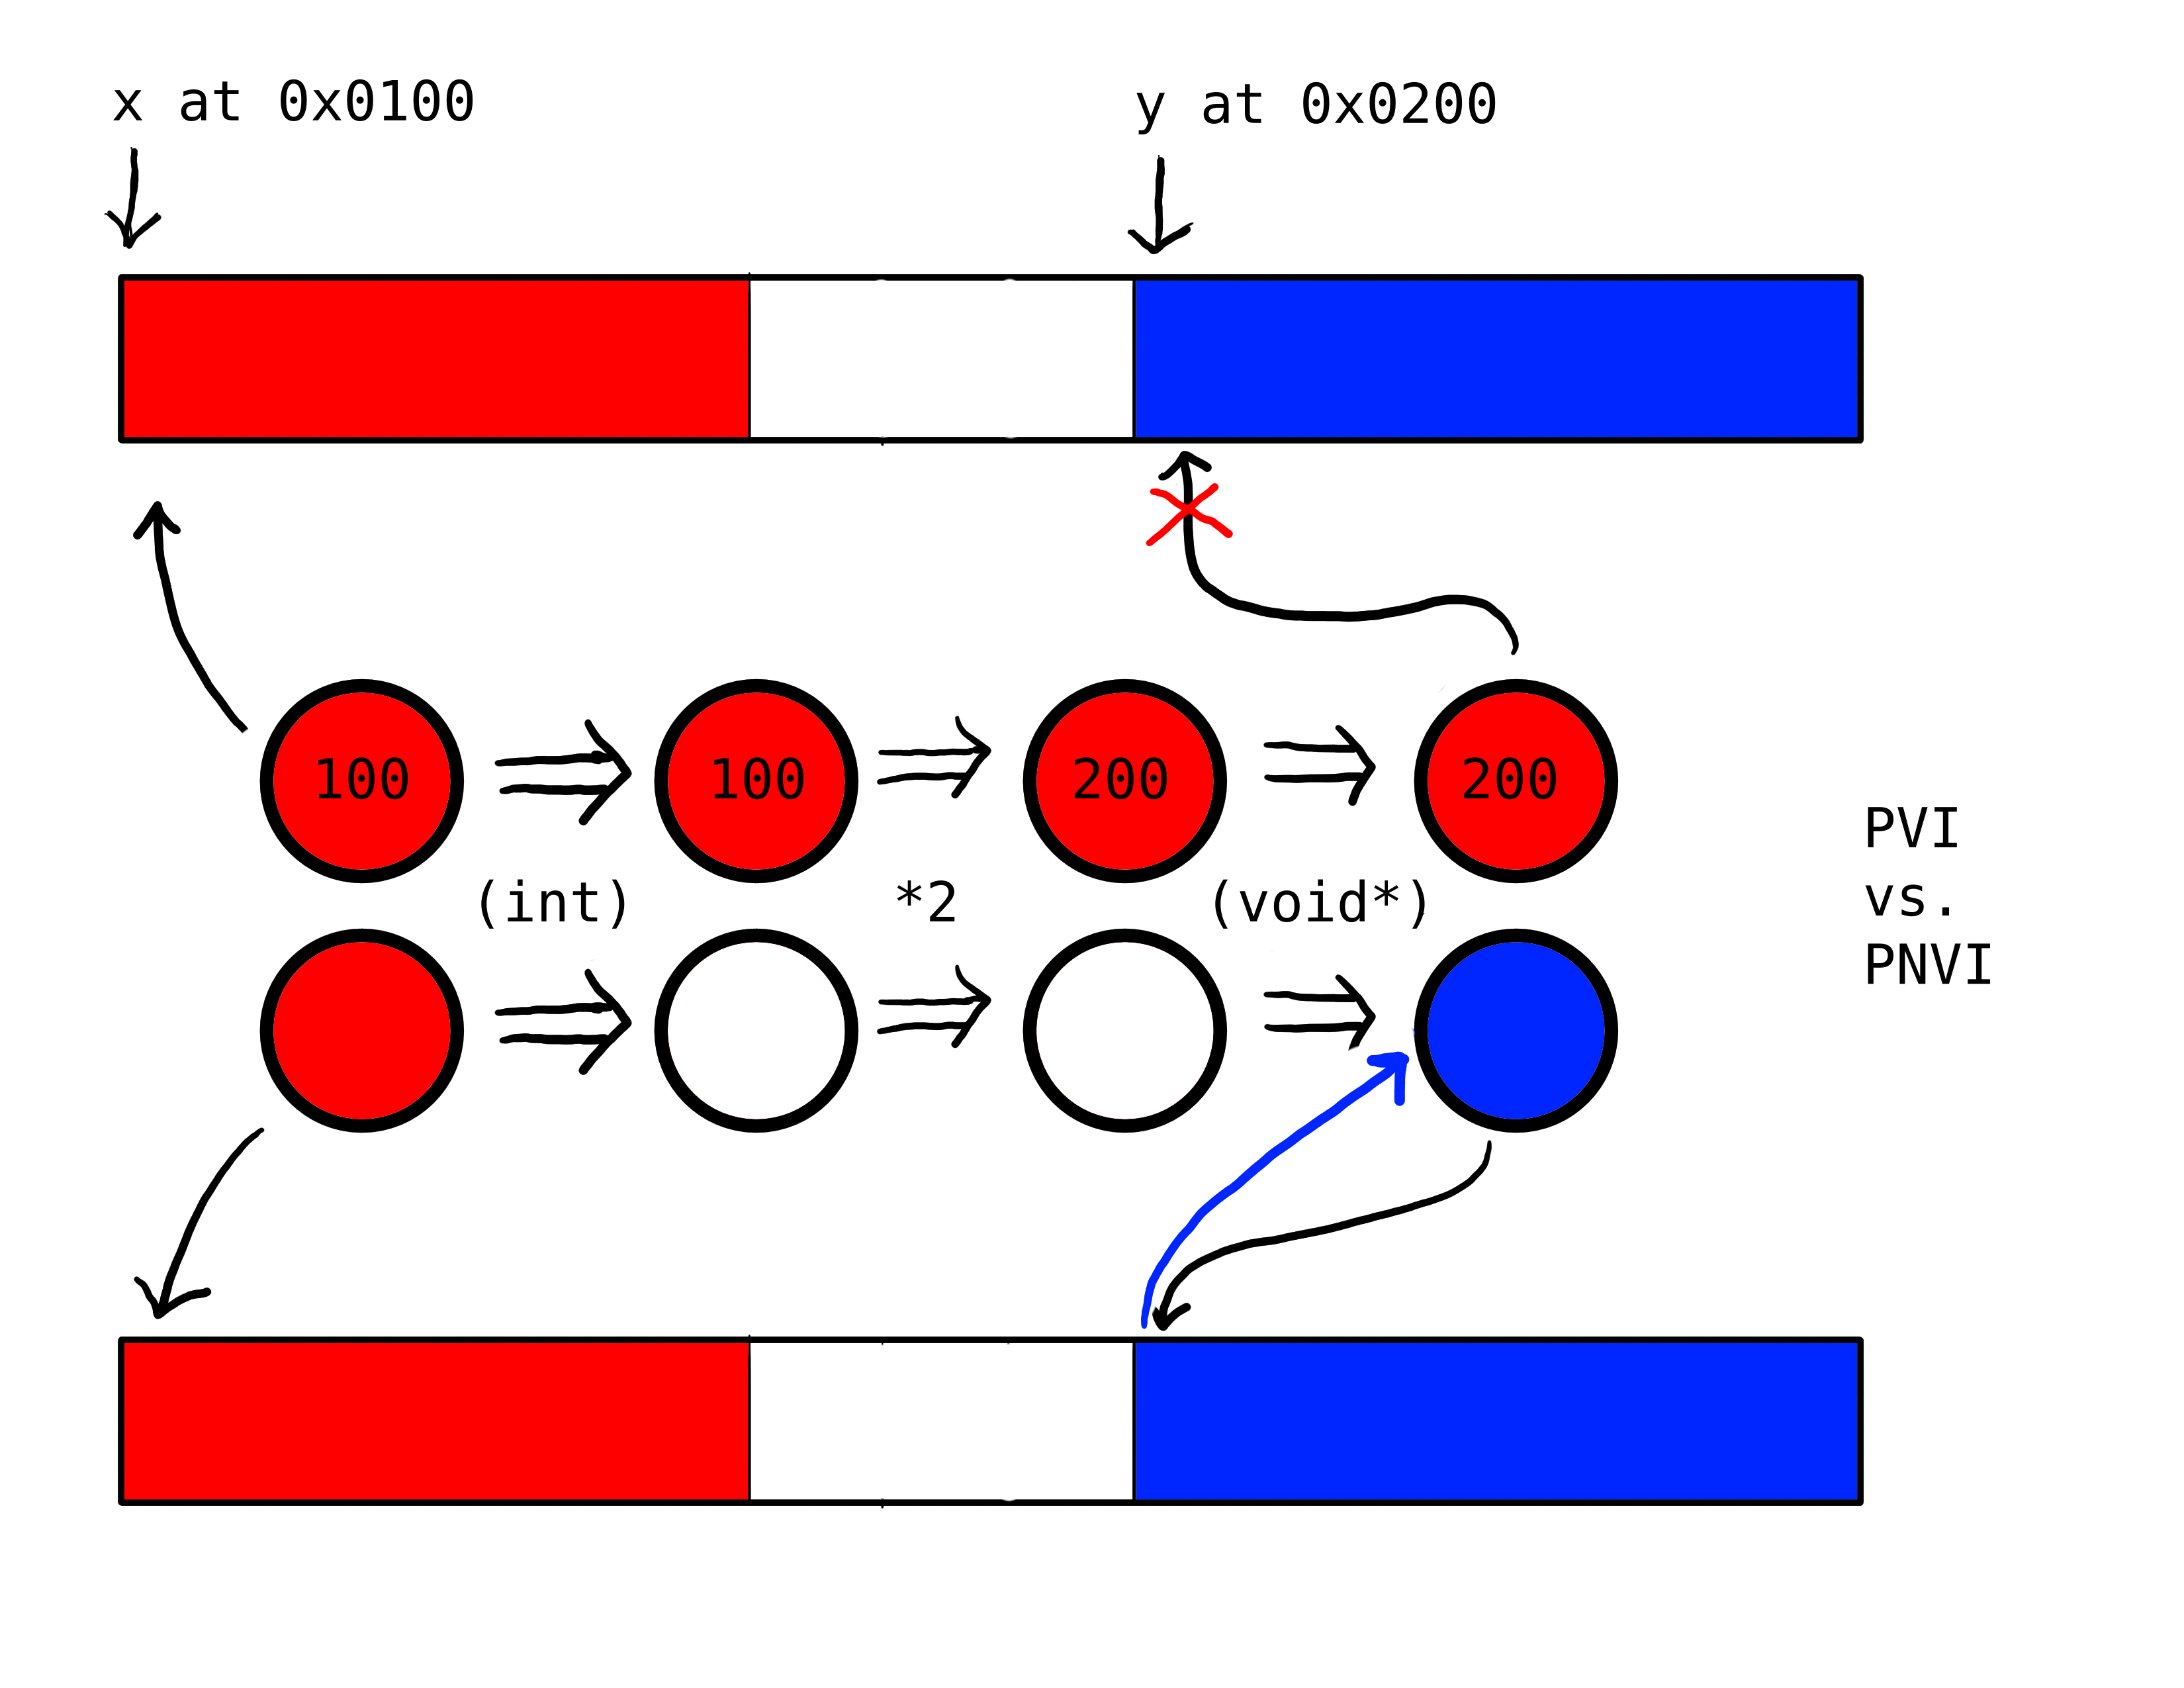
\includegraphics[width=.6\textwidth]{PVIvsPNVI.png}
%  \caption{Integer-pointer casts in PVI and PNVI}
%  \label{fig:PVI-PNVI}
%\end{figure}

%We will aim to prove that for any program, if it is run in both the PVI semantics
%and in Tagged C with our PVI policy, it either produces identical output, or it is both
%undefined in the PVI semantics and failstops in Tagged C. Likewise for PNVI, except that
%some UB in PNVI is non-deterministic, and we only require that it failstop in an execution
%that would {\it reach} the UB.

%In PNVI, the basic provenance model remains the same as PVI, so we can reuse most of the
%same rules. The primary difference is what happens when we cast a pointer to an integer.
%In PVI, tags are propagated as normal.
%To support PNVI, we need the {\it cast} expression to update the tags of a pointer
%being cast to an integer and vice versa. We add two special-case steps to reflect this.

%\judgmenttwo{\optional{\(\mem[p]_{|ty|} = \_@\vt_2 @ \overline{\lt}\)}}
%            {\(\trule{\picasttres}{\picastt}\)}
%            {\(\defestate{\cast{int}{\val{p}{\pt}}}{\tptr{ty}} \longrightarrow
%              \defestate{\val{p}{vt}}{int}\)}

%\judgmenttwo{\optional{\(\mem[p]_{|ty|} = \_@\vt_2 @ \overline{\lt}\)}}
%            {\(\trule{\ipcasttres}{\ipcastt}\)}
%            {\(\defestate{\cast{int}{\val{p}{\pt}}}{\tptr{ty}} \longrightarrow
%              \defestate{\val{p}{vt}}{int}\)}

%For casting an integer to a pointer, we don't need the optional ``peek'' at the memory that it points to.
%We simply clear the tag on the resulting integer. On the other hand, when casting back to a pointer,
%we need to check the color of the object that it points to.

%\begin{minipage}{0.34\textwidth}
%\[\begin{aligned}
%\truledef{\picastt}
%\settag{\PCT'}{\PCT}
%\settag{\vt}{N}
%\end{aligned}\]
%\end{minipage}
%\begin{minipage}{0.65\textwidth}
%\[\begin{aligned}
%\truledef{\ipcastt}
%\assert{\exists t . \forall \lt \in \overline{\lt} . \lt = t \land t \not = N}
%\settag{\PCT'}{\PCT}
%\settag{\pt}{t}
%\end{aligned}\]
%\end{minipage}

%\paragraph{Realizing the Integer-Pointer Cast}

\subsection{Secure Information Flow}
\label{sec:SIF}

Memory safety and compartmentalization both either prevent or mitigate memory errors.
But programs can be memory safe and still do insecure things! Consider the
following code, in which we have some error-handling code that writes to a log.
[TODO: more realistic example]

\begin{verbatim}
int checked_div(int a, int b) {
  if (a % b == 0) {
    return a / b;
  } else {
    fprintf(log, "%d should divide %d but doesn't\n", b, a);
    return 0;
  }
}

void main(int factor) {
  int key = read_and_parse(keyfile);
  int dividend = checked_div(key, factor);
  if (!dividend) { ... } else { ... }
}
\end{verbatim}

The {\tt checked\_div} function sometimes writes its arguments to a log,
which is reasonable enough, except when it's called with a key as an argument!
Suddenly we have keys being written to an unexpected and probably unprotected file.

This is an instance of problematic information-flow. The solution is to implement
a {\em secure information flow} (SIF) policy in Tagged C. SIF is a variant of
{\em information flow control} (IFC) described in the venerable Denning and Denning
\cite{Denning77:SecureInformationFlow}. At its simplest, if we classify inputs and outputs to
the program into secure (``high'') and public (``low'') classifications, then the
high inputs do not influence the low outputs. This generalizes to an arbitrary set
of security classes, but out first example is concerned with just two: the value
returned from {\tt read\_and\_parse} and the output to the log.
In our treatment of this example, we will describe a policy tailored to this particular
set of security classes.

\paragraph*{SIF Example Policy 1}

Let's assume that {\tt read\_and\_parse} is an {\em external} function---that is, we will not
model its internal behavior, so we know nothing about the value it returns. We can therefore
treat that value as an input, and track its influence through the system.

For this initial, simplified policy, we will assume that it is the only input that we care about,
so we have four classes of tags. The default tag \(\N\) represents values that are not tainted
by the sensitive input, the tag \(\vtaint{}\) represents values that have been influenced by
{\tt read\_and\_parse}, and the tag \(\pctaint{f}{\overline{L}}\) carries a set of labels
representing that the current control-flow of the program is tainted (we will discuss this in detail
below.) Lastly, the tag \(\vol\) marks the memory locations of {\em volatile} global variables.
Volatile variables represent mmapped regions or memory that for other reasons is accessible
outside the process.

Initially, the PC Tag is \(\pctaint{f}{\emptyset}\), and all values and memory locations are
tagged \(\N\). The taint tags are introduced at the external call to {\tt read\_and\_parse}.
At the same time, all external calls must check that they aren't leaking a tainted value!

\begin{minipage}{0.25\textwidth}
{ \color{blue}
  \begin{align*}
    \tau ::= & \N \\
    & \vtaint{} \\
    & \pctaint{f}{\overline{L}} \\
    & \vol \\
\end{align*} }
\end{minipage}
\begin{minipage}{0.74\textwidth}
\[\begin{aligned}
\truledef{\extcallt}
\assert{\forall \vt \in \overline{\vt} . \vt = \N \land \PCT = \N}
\settag{\PCT'}{\PCT}
\settag{\vt'}{\caseof{f}}
\caseentry{read\_and\_parse}{\vtaint{}} \\
\caseentry{\_}{\vt} \\
\end{aligned}\]
\end{minipage}

When two values are combined with a binary operation, the resulting value is tainted
if either of them was. We define this as the {\em join} or {\em least-upper-bound}
operator, \(\sqcup\). We will then compare tags according to a partial order, the
{\em no-higher-than} operator, \(\sqsubseteq\). In this case, \(a \sqsubseteq b\)
means that \(a\) does not have higher privilege than \(b\), and so information is
allowed to flow from \(a\) to \(b\).

\begin{minipage}[t]{.49\textwidth}
\[t_1 \sqcup t_2 \triangleq
\begin{cases}
  \vtaint{} & \textnormal{if } t_1 = \vtaint{} \\
  \vtaint{} & \textnormal{if } t_2 = \vtaint{} \\
  \N & \textnormal{otherwise} \\
\end{cases}\]
\end{minipage}
\begin{minipage}[t]{.49\textwidth}
\[t_1 \sqsubseteq t_2 \triangleq
\begin{cases}
  \mathbf{false} & \textnormal{if } t_1 = \vtaint{} \textnormal{ and } t_2 = \vol \\
  \mathbf{true} & \textnormal{otherwise} \\
\end{cases}\]
\end{minipage}

The policy needs to failstop if a tainted value becomes visible to the outside world.
That can happen when the value is passed as an argument to an external function, as we
saw above, or when it is stored to volatile memory (typically representing a file or external
device that might be read or might transfer.

\begin{tikzpicture}
  \binoptruleblock{}{\(\PCT\)}{\(\vt_1 \sqcup \vt_2\)}
\end{tikzpicture}
  
\begin{tikzpicture}
  \storetruleblock{\(\mathbf{assert} ~ \forall \lt \in \lts . \PCT \sqcup \pt \sqcup \vt_2 \sqsubseteq \lt\)}
                  {\(\PCT\)}
                  {\(\PCT \sqcup \pt \sqcup \vt_2\)}
                  {\(\lts\)}
\end{tikzpicture}

Things become trickier when we consider that the program's control-flow itself can be tainted.
This can occur in any of our semantics' steps that can produce different statements and continuations
depending on the tained value. At that point, any change to the machine state constitutes
an information flow. This is termed an {\em implicit flow}.

Implicit flows become much more complex outside of expressions, when we have more
complex control flow. This time the taint is carried on the PC Tag itself.
When the PC Tag is tainted, all stores to memory and all updates to environments must
also be tainted until all branches eventually rejoin, which might be at any point.
We term the point at which it is safe to remove taint a {\it join point}.
In terms of the program's control-flow graph, the
join point of a branch is its immediate post-dominator \cite{}.
[TODO: this is the Denning cited in Bay and Askarov]

In many simple programs, the join point of a conditional or loop is obvious:
the point at which the chosen branch is complete, or the loop has ended.
Such a simple example can be seen in \cref{fig:ifthenelse}; {\tt public1} must be
tagged with the taint tag of {\tt secret}, while it is safe to tag {\tt public2}
\(\N\), because that is after the join point, {\tt J}. The same goes for \cref{fig:while},
if we are in a {\em termination-insensitive} setting \cite{Askarov08:TINILeaks}.
In termination-insensitive noninterference, we allow
an observer to glean information by the termination or non-termination of
the program. So, it is safe to assume that the post-dominator \(J\)
of the while loop is reached.

[TODO: implicit flow rules for statements]

But in the presence of unrestricted go-to statements, a join point may not be
local (and sometimes may not exist within the function, assuming that we have not
consolidated return points.) Consider \cref{fig:forbreak}, which
uses go-to statements to create an approximation of an if-statement whose join-point
is far removed from the for-loop. The label {\tt J} now has nothing to do with the
semantics of any particular statement.

Luckily this can be determined statically from a function's full control-flow graph,
so we can implement it as long as we're willing to deviate from our purely syntax-based
tag rules by performing a code transformation. This can be done completely automatically;
for each split point in the code, the control-flow graph identifies its join point statement,
and the transformation must wrap that statement in a fresh label.

to implement the policy, we must first transform our program
by adding labels at the join point of each conditional.
Every statement that branches carries an optional label indicating its corresponding
join point, if it has one---a function with multiple returns might not, in which case
once the PC Tag is tainted, it must remain so until a return.

\begin{figure}
  \begin{subfigure}{0.4\textwidth}
\begin{verbatim}
int f(bool secret) {
    int public1, public2;

S:  if (secret) {
b1:     public1 = 1;
    } else {
b2:     public1 = 0;
    }

J:  public2 = 42;

    return public2;
}
\end{verbatim}
  \end{subfigure}
  \begin{subfigure}{0.5\textwidth}
    \begin{tikzpicture}
      [ initial text={}, initial distance=4em,
        accepting/.style=accepting by arrow,
        accepting distance=4em
      ]
      \node[state,initial]    (S)                        {$S$};
      \node[state]            (b_1) [above right=of S]   {$b_1$};
      \node[state]            (b_2) [below right=of S]   {$b_2$};
      \node[state,accepting]  (J)   [below right=of b_1] {$J$};

      \path[->] (S)   edge              node  {}  (b_1)
                      edge              node  {}  (b_2)
                (b_1) edge              node  {}  (J)
                (b_2) edge              node  {}  (J);
    \end{tikzpicture}
  \end{subfigure}
  
  \caption{Leaking via if statements}
  \label{fig:ifthenelse}
\end{figure}

\begin{figure}
  \begin{subfigure}{0.4\textwidth}
\begin{verbatim}
int f(bool secret) {
    int public1=1;
    int public2;

S:  while (secret) {
b1:     public1 = 1;
        secret = false;
    }

J:  public2 = 42;

    return public2;
}
\end{verbatim}
  \end{subfigure}
  \begin{subfigure}{0.5\textwidth}
    \begin{tikzpicture}
      [ initial text={}, initial distance=4em,
        accepting/.style=accepting by arrow,
        accepting distance=4em
      ]
      \node[state,initial]    (S)                        {$S$};
      \node[state]            (b_1) [above right=of S]   {$b_1$};
      \node[state,accepting]  (J)   [below right=of b_1] {$J$};

      \path[->] (S)   edge               node  {}  (b_1)
                      edge               node  {}  (J)
                (b_1) edge [bend right] node  {}  (S);
    \end{tikzpicture}
  \end{subfigure}
  
  \caption{Leaking via while statements}
  \label{fig:while}
\end{figure}

\begin{figure}
  \begin{subfigure}{0.25\textwidth}
\begin{verbatim}
int f(bool secret) {
    int public1, public2;

    while (secret) {
        goto b1;
    }

b2: public1 = 1;
    goto J;

b1: public1 = 1;

J:  public2 = 42;
    return public2;
}
\end{verbatim}
  \end{subfigure}
  \begin{subfigure}{0.74\textwidth}
    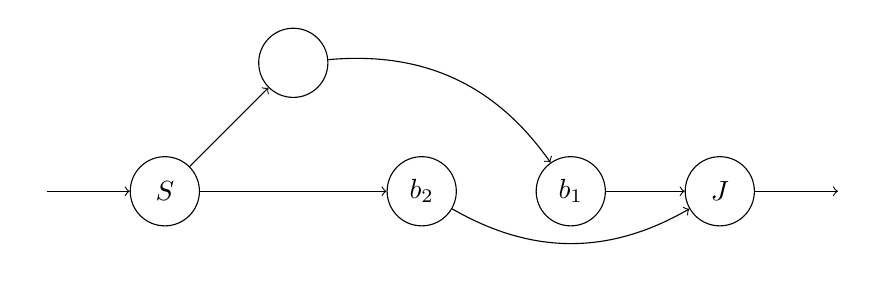
\begin{tikzpicture}
      [ initial text={}, initial distance=3em,
        accepting/.style=accepting by arrow,
        accepting distance=3em
      ]
      \node[state,initial]    (S)                              {$S$};
      \node[state]            (inside) [above right=of S]      {};
      \node[state]            (b_2)    [below right=of inside] {$b_2$};
      \node[state]            (b_1)    [right=of b_2]          {$b_1$};
      \node[state,accepting]  (J)      [right=of b_1]          {$J$};

      \path[->] (S)   edge              node  {}  (inside)
                      edge              node  {}  (b_2)
                (inside) edge [bend left] node {} (b_1)
                (b_1) edge              node  {}  (J)
                (b_2) edge [bend right] node  {}  (J);
    \end{tikzpicture}
  \end{subfigure}
  
  \caption{Cheating with go-tos}
  \label{fig:forbreak}
\end{figure}
\begin{figure}
  \begin{subfigure}{0.3\textwidth}
    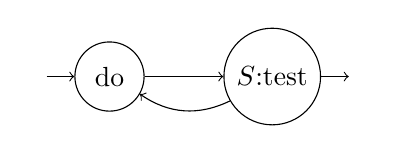
\begin{tikzpicture}
      [ initial text={}, initial distance=1em,
        accepting/.style=accepting by arrow,
        accepting distance=1em
      ]
      \node[state,initial]    (do)                             {do};
      \node[state,accepting]  (S) [right=of do]                {\(S\):test};

      \path[->] (do)   edge              node  {}  (S)
                (S)    edge [bend left]  node  {}  (do);
    \end{tikzpicture}
    \subcaption{Do-while}
  \end{subfigure}
  \begin{subfigure}{0.3\textwidth}
    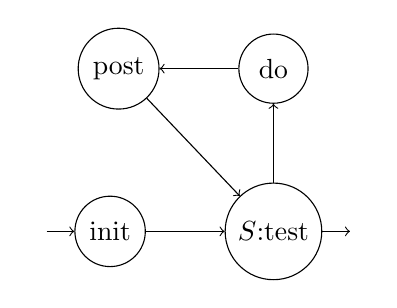
\begin{tikzpicture}
      [ initial text={}, initial distance=1em,
        accepting/.style=accepting by arrow,
        accepting distance=1em
      ]
      \node[state,initial]    (init)                             {init};
      \node[state,accepting]  (S)    [right=of init]             {\(S\):test};
      \node[state]            (do)   [above=of S]                {do};
      \node[state]            (post) [left=of do]                {post};
      
      \path[->] (init)   edge              node  {}  (S)
                (S)      edge              node  {}  (do)
                (do)     edge              node  {}  (post)
                (post)   edge              node  {}  (S);
    \end{tikzpicture}
    \subcaption{For}
  \end{subfigure}
  \begin{subfigure}{0.3\textwidth}
    \center
    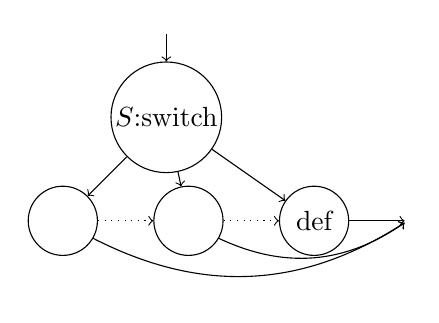
\begin{tikzpicture}
      [ initial text={}, initial distance=1em, initial above,
        accepting/.style=accepting by arrow,
        accepting distance=1em, node distance=2em, inner sep=1pt
      ]
      \node[state,initial]    (switch)                           {\(S\):switch};
      \node[state]            (case1)    [below left=of switch]  {};
      \node[state]            (case2)    [right=of case1]        {};
      \node[state]            (default)  [right=of case2]        {def};
      \node                   (after)    [right=of default]      {};

      \path[->] (switch)  edge              node  {}  (case1)
                          edge              node  {}  (case2)
                          edge              node  {}  (default)
                (default) edge              node  {}  (after)
                (case1)   edge [bend right] node  {}  (after)
                (case2)   edge [bend right] node  {}  (after);

      \path[dotted,->] (case1) edge              node  {}  (case2)
                (case2) edge              node  {}  (default);
                         
    \end{tikzpicture}
    \subcaption{Switch}
  \end{subfigure}
  
  \caption{Remaining Branch Statements}
  \label{fig:rest}
\end{figure}

\paragraph*{Intransitive SIF}

Our second example involves information from outside of the system ending up somewhere it isn't supposed to.

\begin{verbatim}
void sanitize(buf);
char* sql_query(char* query);

void get_data() {
  char[20] name;
  char[100] query = "select address where name =";

  scanf("%19f", name);
  sanitize(name);
  strncat(query, name, strlen(name));
  
  sprintf(buf, sql_query(query));
  return;
}
\end{verbatim}

This function sanitizes its input {\tt name}, then appends the result to an appropriate SQL
query, storing the result in {\tt buf}. But, in the default case, the programmer has accidentally
used the unsanitized string! This creates the opportunity for an SQL injection attack: a caller
to this function could (presumably at the behest of an outside user) call it with {\tt field} of
3 and {\tt name} of ``Bobby; drop table;''.

In this example, we want to implement an {\it intransitive integrity} SIF policy:
we wish to allow {\tt name} to influence the result of {\tt sanitize}, naturally, and the result
of {\tt sanitize} to influence the value passed to {\tt sql\_query}, but we do not wish for
{\tt name} to influence {\tt sql\_query} directly.

In this context, we consider the functions {\tt scanf} and {\tt sanitize} as sources of
information, and the input to {\tt sanitize} and {\tt sql\_query} as information ``sinks.''

Let \(\Sigma\) be the set of these three identifiers, ranged over by \(\sigma\). A value may be tainted
any subset of \(\Sigma\),
written \(\vtaint{\overline{\sigma}}\). The PC Tag tracks the current function identifier and an
association list of labels and sources. Each pair \((L, \sigma)\) in the association list indicates
that until reaching label \(L\), the state itself has been influenced by \(\sigma\).

\[  \color{blue}
\begin{aligned}
  \tau ::= & \vtaint{\overline{id}} \\
  & \pctaint{f}{ets}{\overline{(L,id)}} \\
  & \N \\
\end{aligned}\]

We define the join operation in this new setting, as well as the {\em minus} operation (\(\gentag_1 - \gentag_2\)).
%
\[\gentag_1 \sqcup \gentag_2 \triangleq
\begin{cases}
  \vtaint{(\overline{\sigma}_1 \cup \overline{\sigma}_2)} &
  \textnormal{if } \gentag_1 = \vtaint{\overline{\sigma}_1} \textnormal{ and }
  \gentag_2 = \vtaint{\overline{\sigma}_2}\\
  \vtaint{(\overline{\sigma}_2 \cup \{\sigma \mid (L,\sigma) \in \overline{(L,\sigma)}_1\})} &
  \textnormal{if } \gentag_1 = \pctaint{f}{\overline{(L,\sigma)}_1} \textnormal{ and }
  \gentag_2 = \vtaint{\overline{\sigma}_2}\\
  \vtaint{(\overline{\sigma}_1 \cup \{\sigma \mid (L,\sigma) \in \overline{(L,\sigma)}_2\})} &
  \textnormal{if } \gentag_2 = \pctaint{f}{\overline{(L,\sigma)}_2} \textnormal{ and }
  \gentag_1 = \vtaint{\overline{\sigma}_1}\\
  \bot & \textnormal{otherwise} \\
\end{cases}\]
%
\[\gentag - \sigma \triangleq
\begin{cases}
  \vtaint{\overline{\sigma} - \sigma} &
  \textnormal{if } \gentag = \vtaint ~ \overline{\sigma} \\
  \bot & \textnormal{otherwise} \\
\end{cases}\]

And once again we wish to define the ``no-higher-than'' relation. In this case,
recall that we want to avoid the {\tt name} argument flowing to {\tt sql\_query}.
So we will define that \(\mathtt{sql\_query(query)}\), as a sink, is strictly
higher security than \(\mathtt{sql\_query(name)}\), and every other combination is fine.

\[\gentag_1 \sqsubseteq (\gentag_2,\gentag_3) \triangleq
\begin{cases}
  \mathbf{f} & \textnormal{if } \gentag_1 = \vtaint{\overline{\sigma}},
  \gentag_2 = \mathtt{sql\_query}, \gentag_3 = \mathtt{query}, \textnormal{ and }
  \mathtt{name} \in \overline{\sigma} \\
  \mathbf{t} & \textnormal{otherwise} \\
\end{cases}\]

\paragraph{Tainting and Checking Arguments and Returns}

A function argument or return value can be either a source or a sink.
So, when they are processed by the argument and return rules,
we must both check that the value being passed or returned is not tainted by a forbidden
source, and then add the new source to its taint. Recall that we want the first argument to
the {\tt sanitize} function to ``forget'' the influence of {\tt name}.

\begin{minipage}[t]{.49\textwidth}
  \[\begin{aligned}
  \truledef{\argt}
  \assert{\PCT \sqcup \vt \sqsubseteq (f, x)}
  \letin{\vt_1 := \vt - \{\mathtt{santize(src)}\}}
  \letin{\vt_2 := \vt_1 \sqcup \vtaint{\{f(x)\}}}
  \settag{\vt'}{\vt_2}
  \settag{\PCT'}{\PCT}
  \settag{\lts}{\left[\N\right]}
  \end{aligned}\]
\end{minipage}
\begin{minipage}[t]{.49\textwidth}
  \[\begin{aligned}
  \truledef{\rett}
  \assert{\PCT \sqcup \vt \subseteq \sink{(f.ret)}}
  \letin{\vt_1 := \vt - \{\sigma \mid \sigma / f.ret \in I \}}
  \letin{\vt_2 := \vt_1 \sqcup \mathit{tainted} ~ \{f.ret\}}
  \settag{\vt'}{\vt_2}
  \settag{\PCT'}{\PCT}
  \end{aligned}\]
\end{minipage}

\paragraph{Dynamic Sinks and Globals}

One scenario that does not really match the others is when the sink is dynamically allocated
memory. In this case, we need to tag the memory at allocation-time with the forbidden
sources. Global variables are also possible sources or sinks, so we initialize their
tags to carry this information.

\begin{minipage}[t]{0.49\textwidth}
\[\begin{aligned}
\truledef{\malloct}
\settag{\pt}{\PCT \sqcup \vtaint{\emptyset}}
\settagopt{\vt}{\vtaint{\emptyset}}
\settagopt{\overline{\lt}}{\left[\sink{f.m}\right]}
\settag{\PCT'}{\PCT}
\end{aligned}\]
\end{minipage}
\begin{minipage}[t]{0.49\textwidth}
\[\begin{aligned}
\truledef{\globalt}
\settag{\pt}{\vtaint{\emptyset}}
\settag{\vt}{\vtaint{\{id\}}}
\settag{\overline{\lt}}{\left[\sink{id}\right]}
\end{aligned}\]
\end{minipage}

\paragraph*{PC Tag Taint}

It now becomes slightly more complicated to keep track of the join-point labels
associated with various sources. [TODO: fix the alignment here.]

\begin{minipage}[t]{.25\textwidth}
\[\begin{aligned}
\truledef{\splitt}
\letin{\pctaint{f}{\overline{(L,\sigma)}} := \PCT}
\letin{\vtaint{\sigma} := \vt}
\settag{\PCT'}{\pctaint{f}{(\overline{(L,\sigma)} \cup (L,\sigma))}}
\end{aligned}\]
\end{minipage}
\begin{minipage}[t]{.7\textwidth}
\[\begin{aligned}
\truledef{\labelt}
\letin{\pctaint{f}{\overline{(L,\sigma)}} := \PCT}
\settag{\PCT'}{\pctaint{f}{\{(L',\sigma) \mid (L',\sigma) \in \overline{(L,\sigma)} \land L \not = L'\}}}
\end{aligned}\]
\end{minipage}

The branching constructs are rather complicated, involving multiple steps
and manipulations of the continuation that are not that relevant to their control
points. Rather than give their semantics in full, it suffices to identify which
transitions contain \(\mathbf{SplitT}\) control points. In \cref{fig:rest}, these
are the transitions from the state marked \(S\). Their semantics are given in full
in the appendix.

\paragraph*{Realizing IFC}

In order to implement an IFC policy, we need to specify the rules that it needs to enforce.
The positive here is that the rules are not dependent on one another (with the exception of
declassification rules), and default to permissiveness when no rule is given. We assume that
the user would supply a separate file consisting of a list of triples: the source, the sink,
and the type of rule. This is then translated into the policy.

The other implementation detail to consider are the label tags. These resemble
instruction tags, and that is exactly how they would be implemented: as a special instruction
tag on the appropriate instruction, which might be an existing instruction or a specially
added no-op, that the processor handles by introducing a tag corresponding to that label.

It remains to generate those labels. For purposes of an IFC policy, we first generate the program's
control flow graph. Then, for each if, while, do-while, for, and switch statement, we identify the
immediate post-dominator in the graph, and wrap it in a label statement with a fresh identifier.
That identifier is also added as a field in the original conditional statement. The tags
associated with the labels are initialized at program state---in the case of IFC, these defaults
declare that there are no secrets to lower when it is reached.

\section{Implementing Tagged C with PIPE}

[TODO: more detailed description of Chris' work and why the optional arguments are optional]

\section{Evaluation}
\label{sec:evaluation}

Tagged C aims to combine the flexibility of tag-based architectures with the abstraction
of a high-level language. How well have we achieved this aim?

[Here we list criteria and evaluate how we fulfilled them]

\begin{itemize}
\item Flexibility: we demonstrate three policies that can be used alone or in conjunction
\item Applicability: we support the full complement of C language features and give definition
  to many undefined C programs
\item Practical security: our example security policies are based on important security concepts
  from the literature
\end{itemize}

\subsection{Limitations of the Tag Mechanism}

By committing to a tag-based mechanism, we do restrict the space of policies that Tagged C
can enforce. In general, a reference monitor can enforce any policy that constitutes a
{\em safety property}---any policy whose violation can be demonstrated by a single finite
trace. This class includes such policies as ``no integer overflow'' and ``pointers are always in-bounds,''
which depend on the values of variables. Tag-based monitors cannot enforce any policy that
depends on the value of a variable rather than its tags.

\section{Related Work}

\paragraph{Reference Monitors}

The concept of a reference monitor was first introduced fifty years ago in \cite{Anderson72:PlanningStudy}:
a tamper-proof and verifiable subsystem that checks every security-relevant operation in a system to
ensure that it conforms to a security {\em policy} (a general specification of acceptable behavior;
see \cite{Goguen82:SecurityPolicies}.)

A reference monitor can be implemented at any level of a system. An {\em inline reference monitor}
is a purely compiler-based system that inserts checks at appropriate places in the code.
Alternatively, a reference monitor might be embedded in the operating system, or in an interpreted
language's runtime. A {\em hardware reference monitor} instead provides primitives at the ISA-level
that accelerate security and make it harder to subvert.

Programmable Interlocks for Policy Enforcement (PIPE) \cite{Dhawan14:PUMP} is a hardware extension
that uses {\em metadata tagging}. Each register and each word of memory is associated with
an additional array of bits called a tag. The policy is decomposed into a set of {\em tag rules}
that act in parallel with each executing instruction, using the tags on its operands to
decide whether the instruction is legal and, if so, determine which tags to place on its results.
PIPE tags are large relative to other tag-based hardware, giving it the flexibility
to implement complex policies with structured tags, and even run multiple policies at once.

Other hardware monitors include Arm MTE, [Binghamton], and CHERI.
Arm MTE aims to enforce a narrow form of memory safety using 4-bit tags, which distinguish adjacent objects
in memory from one another, preventing buffer overflows, but not necessarily other memory violations.
[TODO: read the Binghamton paper, figure out where they sit here.] 

CHERI is capability machine [TODO: cite OG CHERI]. In CHERI, capabilities
are ``fat pointers'' carrying extra bounds and permission information, and capability-protected
memory can only be accessed via a capability with the appropriate privilege. This is a natural
way to enforce spatial memory safety, and techniques have been demonstrated for enforcing
temporal safety \cite{NWF20:Cornucopia}, stack safety \cite{Skorstengaard19:stktokens},
and compartmentalization [TODO: figure out what to cite], with varying degrees of ease and
efficiency. But CHERI cannot easily enforce notions of security based on dataflow,
such as Secure Information Flow.

In this paper, we describe a programming language with an abstract reference monitor.
We realize it as an interpreter with the reference monitor built in, and envision
eventually compiling to PIPE-equipped hardware. An inlining compiler would also be plausible.
As a result of this choice, our abstract reference monitor uses a PIPE-esque notion of
tags.

\paragraph{Aspect Oriented Programming}

[TODO: do forward search from original AOP paper]

\section{Future Work}
\label{sec:futurework}

We have presented the language and a reference interpreter, built on top of the CompCert interpreter
\cite{Leroy09:CompCert}, and three example policies. There are several significant next-steps.

\paragraph{Compilation}

An interpreter is all well and good, but a compiler would be preferable for many reasons.
A compiled Tagged C could use the hardware acceleration of a PIPE target, and could more easily
support linked libraries, including linking against code written in other languages.
The ultimate goal would be a fully verified compiler, but that is a very long way off.

\paragraph{Language Proofs}

There are a couple of properties of the language semantics itself that we would like to prove.
Namely (1) that its behavior (prior to adding a policy) matches that of CompCert C and
(2) that the behavior of a given program is invariant under all policies up to truncation due
to failstop.

\paragraph{Policy Correctness Proofs}

For each example policy discussed in this paper, we sketched a formal specification for the
security property it ought to enforce. A natural continuation would be to prove the correctness
of each policy against these specifications.

\paragraph{Policy DSL}

Currently, policies are written in Gallina, the language embedded in Coq. This is fine for a
proof-of-concept, but not satisfactory for real use. We plan to develop a domain-specific policy
language to make it easier to write Tagged C policies.

\bibliographystyle{splncs04}
\bibliography{taggedc.bib}

\appendix

\section{Syntax}

\begin{figure}
  \begin{subfigure}[t]{0.3\textwidth}
    \[\begin{aligned}
    \stmt ::= & \sskip \\
    | & \sdo{\expr} \\
    | & \sseq{\stmt_1}{\stmt_2} \\
    | & \sifthenelse{\expr}{\stmt_1}{\stmt_2}{L} \\
    | & \swhile{\expr}{\stmt}{L} \\
    | & \sdowhile{\expr}{\stmt}{L} \\
    | & \sfor{\stmt_1}{\expr}{\stmt_2}{\stmt_3} \\
    | & \sbreak \\
    | & \scontinue \\
    | & \sreturn \\
    | & \sswitch{\expr}{\overline{(L,\stmt)}} \\
    | & \slabel{L}{\stmt} \\
    | & \sgoto{L} \\    
    \end{aligned}\]
  \end{subfigure}
  \begin{subfigure}[t]{0.69\textwidth}
    \[\begin{aligned}
    \expr ::= & \val{v}{\vt} & \textnormal{Value} \\
    | & \var{x} & \textnormal{Variable} \\
    | & \field{\expr}{id} & \textnormal{Field} \\
    | & \valof{\expr} & \textnormal{Load from Object} \\
    | & \deref{\expr} & \textnormal{Dereference Pointer} \\
    | & \addrof{\expr} & \textnormal{Address of Object} \\
    | & \unop{\odot}{\expr} & \textnormal{Unary Operator} \\
    | & \binop{\oplus}{\expr_1}{\expr_2} & \textnormal{Binary Operator} \\
    | & \cast{\expr}{ty} & \textnormal{Cast} \\
    | & \condition{\expr_1}{\expr_2}{\expr_3} & \textnormal{Conditional} \\
    | & \sizeof{ty} & \textnormal{Size of Type} \\
    | & \alignof{ty} & \textnormal{Alignment of Type} \\
    | & \assign{\expr_1}{\expr_2} & \textnormal{Assignment} \\
    | & \assignop{\oplus}{\expr_1}{\expr_2} & \textnormal{Operator Assignment} \\
    | & \postinc{\oplus}{\expr} & \textnormal{Post-Increment/Decrement} \\
    | & \comma{\expr_1}{\expr_2} & \textnormal{Expression Sequence} \\
    | & \call{\expr_f}{\overline{\expr}_{args}} & \textnormal{Function Call} \\
    | & \loc{l}{\lt} & \textnormal{Memory Location} \\
    | & \paren{\expr}{ty}{\gentag} & \textnormal{Parenthetical with Optional Cast} \\
    \end{aligned}\]
  \end{subfigure}
  \caption{Tagged C Abstract Syntax}
  \label{fig:syntax}
\end{figure}

\section{Continuations}
\label{app:continuations}

\[\begin{split}
\cont ::= & \kemp \\
| & \kdo{\cont} \\
| & \kseq{\stmt}{\cont} \\
| & \kif{\stmt_1}{\stmt_2}{L}{\cont} \\
| & \kwhiletest{\expr}{\stmt}{L}{\cont} \\
| & \kwhileloop{\expr}{\stmt}{L}{\cont} \\
| & \kdowhiletest{\expr}{\stmt}{L}{\cont} \\
| & \kdowhileloop{\expr}{\stmt}{L}{\cont} \\
| & \kfor{\expr}{\stmt_2}{\stmt_3}{L}{\cont} \\
| & \kforpost{\expr}{\stmt_2}{\stmt_3}{L}{\cont} \\
\end{split}\]

\section{Initial State}

Given a list \(xs\) of variable identifiers \(id\) and types
\(ty\), a program's initial memory is defined by iteratively allocating each one
in memory and updating the global environment with its base address, bound, type,
and a static identity tag. Let \(|ty|\) be a function from types to their sizes
in bytes. The memory is initialized \(\vundef@\vt@\overline{\lt}\)
for some \(\vt\) and \(\overline{\lt}\), unless given an initializer.
Let \(\mem_0\) and \(\genv_0\) be the initial (empty) memory and environment.
The parameter \(b\) marks the start of the global region.

%Since we don't need to initialize tags in memory dynamically, our rule for
%selecting these tags can cover the entire initialization of the memory with arbitrary
%granularity. We represent this as a list of tags of length \(|ty|\).

\[\mathit{globals} ~ xs ~ b =
\begin{cases}
  (\mem_0, \genv_0) & \textnormal{if } xs = \varepsilon \\
  (\mem[p \dots p+|ty| \mapsto \vundef@\vt@\overline{\lt}]_{|ty|}, & \textnormal{if } xs = (id,ty)::xs' \\
  ~ \genv[id \mapsto (\mathit{p, p+|ty|,ty,\pt})]) & \textnormal{and } \trule{\globaltres}{\globalt} \\
  & \textnormal{where } (\mem,\genv) = \mathit{globals} ~ xs' ~ (b + |ty|) \\
\end{cases}\]

\section{Step Rules}
\label{app:rules}

\subsection{Sequencing rules}

\sequencing

\subsection{Conditional rules}

\conditionals

\subsection{Loop rules}

\loops

\subsection{Contexts}
\label{app:contexts}

Our expression semantics are contextual. A context \(\mathit{ctx}\) is a function from an
expression to an expression and a tag. We identify a valid context using the \(\mathit{context}\)
relation over a ``kind'' (left-hand or right-hand, \(\lh\) or \(\rh\)),
and an expression.

\[\begin{aligned}
\mathit{context} & ~ k ~ \ctx{\expr} ::= \\
| & \mathit{context} ~ k ~ \lambda \expr.\expr & \\ % ctx_top
| & \mathit{context} ~ \lh ~ \lambda \expr.\deref{\ctx{\expr}} &
\textnormal{where } \mathit{context} ~  \rh ~ \ctx{\expr} \\ % ctx_deref
| & \mathit{context} ~ \lh ~ \lambda \expr.\field{\ctx{\expr}}{id} &
\textnormal{where } \mathit{context} ~  \rh ~ \ctx{\expr} \\ % ctx_field
| & \mathit{context} ~ \rh ~ \lambda \expr.\valof{\ctx{\expr}} &
\textnormal{where } \mathit{context} ~  \lh ~ \ctx{\expr} \\ % ctx_rvalof
| & \mathit{context} ~ \rh ~ \lambda \expr.\addrof{\ctx{\expr}} & \textnormal{where } \mathit{context} ~  \lh ~ \ctx{\expr} \\ % ctx_addrof
| & \mathit{context} ~ \rh ~ \lambda \expr.\unop{\odot}{\ctx{\expr}} & \textnormal{where } \mathit{context} ~  \rh ~ \ctx{\expr} \\ % ctx_unop
| & \mathit{context} ~ \rh ~ \lambda \expr.\binop{\oplus}{\ctx{\expr_1}}{\expr_2} & \textnormal{where } \mathit{context} ~  \rh ~ \ctx{\expr_1} \\ % ctx_binop_left
| & \mathit{context} ~ \rh ~ \lambda \expr.\binop{\oplus}{\expr_1}{\ctx{\expr_2}} & \textnormal{where } \mathit{context} ~  \rh ~ \ctx{\expr_2} \\ % ctx_binop_right
| & \mathit{context} ~ \rh ~ \lambda \expr.\cast{\ctx{\expr}}{\type} & \textnormal{where } \mathit{context} ~  \rh ~ \ctx{\expr} \\ % ctx_cast
| & \mathit{context} ~ \rh ~ \lambda \expr.\seqand{\ctx{\expr_1}}{\expr_2} & \textnormal{where } \mathit{context} ~  \rh ~ \ctx{\expr_1} \\ % ctx_seqand
| & \mathit{context} ~ \rh ~ \lambda \expr.\seqor{\ctx{\expr_1}}{\expr_2} & \textnormal{where } \mathit{context} ~  \rh ~ \ctx{\expr_1} \\ % ctx_seqor
| & \mathit{context} ~ \rh ~ \lambda \expr.\condition{\ctx{\expr_1}}{\expr_2}{\expr_3} & \textnormal{where } \mathit{context} ~  \rh ~ \ctx{\expr_1} \\ % ctx_condition
| & \mathit{context} ~ \rh ~ \lambda \expr.\assign{\ctx{\expr_1}}{\expr_2} & \textnormal{where } \mathit{context} ~  \lh ~ \ctx{\expr_1} \\ % ctx_assign_left
| & \mathit{context} ~ \rh ~ \lambda \expr.\assign{\expr_1}{\ctx{\expr_2}} & \textnormal{where } \mathit{context} ~  \rh ~ \ctx{\expr_2} \\ % ctx_assign_right
| & \mathit{context} ~ \rh ~ \lambda \expr.\assignop{\oplus}{\ctx{\expr_1}}{\expr_2} & \textnormal{where } \mathit{context} ~ \lh ~ \ctx{\expr_1} \\ % ctx_assignop_left
| & \mathit{context} ~ \rh ~ \lambda \expr.\assignop{\oplus}{\expr_1}{\ctx{\expr_2}} & \textnormal{where } \mathit{context} ~ \rh ~ \ctx{\expr_2} \\ % ctx_assignop_right
| & \mathit{context} ~ \rh ~ \lambda \expr.\postinc{\oplus}{\ctx{\expr}} & \textnormal{where } \mathit{context} ~  \lh ~ \ctx{\expr} \\ % ctx_postinc
| & \mathit{context} ~ \rh ~ \lambda \expr.\call{\ctx{\expr_1}}{\overline{\expr_2}} & \textnormal{where } \mathit{context} ~  \rh ~ \ctx{\expr_1} \\ % ctx_call_left
| & \mathit{context} ~ \rh ~ \lambda \expr.\call{\expr_1}{\ctx{\overline{\expr_2}}} & \textnormal{where } \mathit{context} ~  \rh ~ \ctx{\expr} \textnormal{ for } \expr \in \overline{\expr_2} \\ % ctx_call_right
% skipped builtins
| & \mathit{context} ~ \rh ~ \lambda \expr.\comma{\ctx{\expr_1}}{\expr_2} & \textnormal{where } \mathit{context} ~  \rh ~ \ctx{\expr_1} \\ % ctx_comma
| & \mathit{context} ~ \rh ~ \lambda \expr.\paren{\ctx{\expr}}{\type}{} & \textnormal{where } \mathit{context} ~  \rh ~ \ctx{\expr} \\ % ctx_paren
| & \mathit{context} ~ \rh ~ \lambda \expr.\paren{\ctx{\expr}}{\type}{\gentag} & \textnormal{where } \mathit{context} ~ \rh ~ \ctx{\expr} \\ % ctx_paren
\end{aligned}\]

Next, we define a notion of expression reduction. A left-hand reduction relates an expression to an expression.
A right-hand reduction relates a triple of PC Tag, memory, and expression to another such triple.

%triple of a memory, an expression, and a tag
%might reduces to another such triple as a left-hand, right-hand, or call reduction, written
%\((\mem, \expr, \PCT) \Rightarrow_k (\mem', \expr', \PCT')\),
%based on rules given below. These reductions are embedded in states as follows.

\judgmenttwo{\(\mathit{context} ~ \lh ~ \ctx{\expr}\)}
            {\(\expr \Rightarrow_\lh \expr'\)}
            {\(\defestate{\ctx{\expr}} \longrightarrow \defestate{\ctx{\expr}}\)}

\judgmenttwo{\(\mathit{context} ~ \rh ~ \ctx{\expr}\)}
            {\((\PCT, \mem, \expr) \Rightarrow_\rh (\PCT', \mem', \expr')\)}
            {\(\defestate{\ctx{\expr}} \longrightarrow \estate{\PCT'}{\mem'}{\ctx{\expr}}{\cont}\)}
            
\subsection{Expression Rules}

\expressions

\subsection{Call and Return Rules}

In order to make a call, we need to reduce the function expression to an \(\floc{\_}\) value, an
abstract location corresponding to a particular function. Then we can make the call.

\callexprstep

When we make an internal call, we need to allocated space for locals and arguments using the helper function
\(\mathit{frame}\).

\[\mathit{frame} ~ xs ~ as ~ \mem =
\begin{cases}
  (\mem''[p \mapsto \vundef@\vt@\overline{\lt}]_{|ty|}, & \textnormal{if } xs = (id,ty)::xs' \\
  \lenv'[id \mapsto (\mathit{p, p+|ty|,ty,\pt})]) &
  \textnormal{where } (\mem',p) \leftarrow \mathit{stack\_alloc} ~ |ty| ~ \mem, \\
  & \trule{\localtres}{\localt}, \\
  & \textnormal{and } (\mem'',\lenv') = \mathit{frame} ~ xs' ~ as ~ m' \\ 
  \\
  (\mem''[p \mapsto v@\vt'@\overline{\lt}]_{|ty|}, & \textnormal{if } as = (id,ty,v @ \vt)::as' \textnormal{ and } xs = \varepsilon \\
  \lenv'[id \mapsto (\mathit{p, p+|ty|,ty,\pt})]) &
  \textnormal{where } (\mem',p) \leftarrow \mathit{stack\_alloc} ~ |ty| ~ \mem, \\
  & \trule{\argtres}{\argt}, \\
  & \textnormal{and } (\mem'',\lenv') = \mathit{frame} ~ xs' ~ as ~ m' \\
  \\
  (\mem, \lambda x . \bot) & \textnormal{if } xs = \varepsilon \textnormal{ and } as = \varepsilon \\
\end{cases}\]

\callstep

On the other hand, when we make an external call, we step directly to a return state with some value
being returned and an updated memory. [TODO: talk more about how the tag policy applies in external
  functions, what they can and can't do with tags.]

\extcallstep

Special external functions, such as malloc, just get their own rules.

\mallocstep

And finally, we have the return rules.

\returnstep
\retvalstep
\retnovalstep

\end{document}
